%%%%%%%%%%%%%%%%%%%%%%%%%%%%%%%%%%%%%%%%%%%%%%%%%%%%%%%%%%%%%%%%%%%%%%%%%%%%%%%%
% Template for USENIX papers.
%
% History:
%
% - TEMPLATE for Usenix papers, specifically to meet requirements of
%   USENIX '05. originally a template for producing IEEE-format
%   articles using LaTeX. written by Matthew Ward, CS Department,
%   Worcester Polytechnic Institute. adapted by David Beazley for his
%   excellent SWIG paper in Proceedings, Tcl 96. turned into a
%   smartass generic template by De Clarke, with thanks to both the
%   above pioneers. Use at your own risk. Complaints to /dev/null.
%   Make it two column with no page numbering, default is 10 point.
%
% - Munged by Fred Douglis <douglis@research.att.com> 10/97 to
%   separate the .sty file from the LaTeX source template, so that
%   people can more easily include the .sty file into an existing
%   document. Also changed to more closely follow the style guidelines
%   as represented by the Word sample file.
%
% - Note that since 2010, USENIX does not require endnotes. If you
%   want foot of page notes, don't include the endnotes package in the
%   usepackage command, below.
% - This version uses the latex2e styles, not the very ancient 2.09
%   stuff.
%
% - Updated July 2018: Text block size changed from 6.5" to 7"
%
% - Updated Dec 2018 for ATC'19:
%
%   * Revised text to pass HotCRP's auto-formatting check, with
%     hotcrp.settings.submission_form.body_font_size=10pt, and
%     hotcrp.settings.submission_form.line_height=12pt
%
%   * Switched from \endnote-s to \footnote-s to match Usenix's policy.
%
%   * \section* => \begin{abstract} ... \end{abstract}
%
%   * Make template self-contained in terms of bibtex entires, to allow
%     this file to be compiled. (And changing refs style to 'plain'.)
%
%   * Make template self-contained in terms of figures, to
%     allow this file to be compiled. 
%
%   * Added packages for hyperref, embedding fonts, and improving
%     appearance.
%   
%   * Removed outdated text.
%
%%%%%%%%%%%%%%%%%%%%%%%%%%%%%%%%%%%%%%%%%%%%%%%%%%%%%%%%%%%%%%%%%%%%%%%%%%%%%%%%

\documentclass[letterpaper,twocolumn,10pt]{article}
\usepackage{usenix2019_v3}

\usepackage{subcaption}
\usepackage{booktabs} % For formal tables
\usepackage[linesnumbered,vlined,ruled]{algorithm2e}
\usepackage{amsmath,amssymb,amsfonts}
\DeclareMathOperator*{\argmax}{arg\,max}
\DeclareMathOperator*{\mean}{mean}
% Copyright
%\setcopyright{none}
%\setcopyright{acmcopyright}
%\setcopyright{acmlicensed}
%\setcopyright{rightsretained}
%\setcopyright{usgov}
%\setcopyright{usgovmixed}
%\setcopyright{cagov}
%\setcopyright{cagovmixed}
\usepackage{mathtools}
\usepackage{multirow}
\usepackage{tikz}
\usepackage[compact]{titlesec}
\usepackage{enumitem}
\setlist[enumerate]{itemsep=0mm}

\DeclarePairedDelimiter\ceil{\lceil}{\rceil}
\DeclarePairedDelimiter\floor{\lfloor}{\rfloor}
%\DeclarePairedDelimiter\parentheses{\(}{\)}

\newif\ifstartedinmathmode
\newcommand\encircled[1]{%
  \relax\ifmmode\startedinmathmodetrue\else\startedinmathmodefalse\fi%
  \tikz[baseline,anchor=base]{%
  \node[draw,circle,outer sep=0pt,inner sep=.2ex]
    {\ifstartedinmathmode$#1$\else#1\fi};}%
}

% inlined bib file
\usepackage{filecontents}

%-------------------------------------------------------------------------------
\begin{filecontents}{\jobname.bib}
%-------------------------------------------------------------------------------
@Book{arpachiDusseau18:osbook,
  author =       {Arpaci-Dusseau, Remzi H. and Arpaci-Dusseau Andrea C.},
  title =        {Operating Systems: Three Easy Pieces},
  publisher =    {Arpaci-Dusseau Books, LLC},
  year =         2015,
  edition =      {1.00},
  note =         {\url{http://pages.cs.wisc.edu/~remzi/OSTEP/}}
}
@InProceedings{waldspurger02,
  author =       {Waldspurger, Carl A.},
  title =        {Memory resource management in {VMware ESX} server},
  booktitle =    {USENIX Symposium on Operating System Design and
                  Implementation (OSDI)},
  year =         2002,
  pages =        {181--194},
  note =         {\url{https://www.usenix.org/legacy/event/osdi02/tech/waldspurger/waldspurger.pdf}}}
\end{filecontents}

%-------------------------------------------------------------------------------
\begin{document}
%-------------------------------------------------------------------------------

%don't want date printed
\date{}

% make title bold and 14 pt font (Latex default is non-bold, 16 pt)
\title{\Large \bf Revealing Privacy Leakage in 3D Mixed Reality Data}

%for single author (just remove % characters)
%\author{
%{\rm Your N.\ Here}\\
%Your Institution
%\and
%{\rm Second Name}\\
%Second Institution
% copy the following lines to add more authors
% \and
% {\rm Name}\\
%Name Institution
%} % end author

\author{
Anonymous Author(s)
%{\rm Jaybie Agullo de Guzman}\\
%Data 61 \&
%University of New South Wales \\
%jaybie.deguzman@data61.csiro.au
%\and
%{\rm Kanchana Thilakarathna}\\
%University of Sydney\\
%kanchana.thilakarathna@sydney.edu.au
%\and
%{\rm Aruna Seneviratne}\\
%University of New South Wales\\
%a.seneviratne@unsw.edu.au
}


\maketitle

%-------------------------------------------------------------------------------
\begin{abstract}
%-------------------------------------------------------------------------------
We have seen a rise in \textit{mixed} (MR) and \textit{augmented reality} (AR) applications and devices in recent years. Subsequently, we have become familiar with the sensing power of these applications and devices, and we are only starting to realize the nascent risks that these technology puts over our privacy and security. Current privacy protection measures are primarily aimed towards known and well-utilised data types (i.e. location, on-line activity, biometric, and so on) while a few works have focused on looking into the security and privacy risks of and providing protection on MR data, particularly on 3D MR data. In this paper, we reveal the privacy leakage from raw 3D MR data and how they persist even after implementing spatial generalizations and abstractions. %; \textcolor{red}{thus, these approaches, especially RANSAC or similar plane generalizations, cannot be used for privacy protection.}
Firstly, we formalize the \textit{spatial} privacy problem in 3D mixed reality data as well as the adversary model. Then, we demonstrate through an inference model how adversaries can identify and potentially reconstruct 3D spaces. Moreover, we also demonstrate how compact these 3D representations can be in terms of memory usage which allows adversaries to create lightweight 3D inference models for user spaces.
\end{abstract}

%\titlespacing{\section}{0pt}{5pt}{3pt}
%\titlespacing{\subsection}{0pt}{3pt}{2pt}
%\titlespacing{\subsubsection}{0pt}{2pt}{1pt}

\section{Introduction}
%MR applications, devices; support from companies like Google and Apple which has significant mobile market share. ARCore, ARKit, and the Windows MR development kit.
Pok\'emon Go's release in 2016 arguably marked the beginning of augmented reality (AR) and mixed reality (MR) to be part of the mainstream mobile market. Although there were numerous earlier applications and devices that already delivered these `reality' experiences, it was only then when significant attention was given to the technology by consumers and companies alike. Soon after, Apple launched the ARKit\footnote{https://developer.apple.com/documentation/arkit} in 2017 and, halfway through 2018, Google followed with the ARCore\footnote{https://developers.google.com/ar/}. Microsoft, on the other hand, focused on the head-mounted displays (or HMDs) with the Hololens and other OEM headsets running their Windows Mixed Reality platform\footnote{https://developer.microsoft.com/en-us/windows/mixed-reality}. These developments undoubtedly signifies the very near future with AR and MR\footnote{From this point onwards, following Milgram's definition\cite{milgram1994taxonomy}, we will be collectively calling both augmented and mixed reality as mixed reality or MR.}.

%Currently, these their use of 3D pointclouds to represent the physical space --> use this to inform where to put augmentations and 'lock' or anchor the augmentations.
To deliver \textit{realistic} augmentations, collected environment sensing information are processed to create an understanding of the physical world and render the augmentations accordingly. Most mobile MR development platforms utilise a form of \textit{visual odometry} \cite{yousif2015overview} combined with motion or inertial information to map the device's position relative to the real-world, while dedicated HMDs, such as the Hololens, leverage multiple cameras with depth sensor/s to understand the environment and create a virtual 3D map. Once a good mapping has been created, the virtual space (or coordinate system) is shared with applications to allow the synthetic or augmented content to interact with the physical world. This mapping is usually in the form of a 3D \textit{point cloud} with some APIs (i.e. Windows MR) including normal vectors to signify orientation of the points which allows for easier surface detection. %Discuss the risks

However, this environment understanding capability required by MR poses unforeseen privacy risks for users. Once these captured 3D maps have been revealed to adversaries, it discloses potentially sensitive spatial information about the user's space and may further be used to inflict harm. Adversaries can vary from a background service that delivers unsolicited ads based on the objects detected from the user's surroundings to burglars who are able to map the user's house based on the released 3D data. Furthermore, turning off GPS tracking for location privacy may no longer be sufficient once the user starts using MR applications that can expose their locations with higher specificity from the visual and 3D data that are exposed\footnote{For example, Google has unveiled their \textit{Visual Positioning Service} (or VPS) using 3D data to locate users in space -- an offshoot of Project Tango -- during their 2018 I/O keynote event.}.

%\paragraph{Motivating Example} Say, a user continues to move around with an MR application which continuously collects 3D information of the real-world. The application can store these data, then stitch and reconstruct the user's real-world space in the form of an \textit{oriented 3D point cloud}. This 3D mapping of oriented points allows the applications to anchor virtual augmentations that stay in place and look seemingly part of the real-world. The mapping also allows interactions with the users and other real-world objects with virtual reactions that follow the laws of physics (such as bouncing or falling due to gravity). 

%Also, most of the time 3D point-clouds are much lighter weight than images or videos due to its sparsity; thus, keeping point-clouds per user may not be as monumental than keeping images and videos.

The recent EU-GDPR ruling aims to address these issues from a policy approach. It aims to empower the users and protect their data privacy by enforcing data protection laws for organizations and companies that handle user data. This highlights the importance of designing and developing \textit{privacy-enhancing technologies} (or PETs). %While the GDPR can be considered as the most important change in data privacy regulation,
Currently, there are numerous PETs designed for structured data (e.g. biometric, personal financial, location, etc.) such as \textit{k}-anonymity \cite{sweeney2002k}, and \textit{differential privacy} \cite{mcsherry2007mechanism, dwork2014algorithmic, erlingsson2014rappor}, as well as techniques for data aggregation during information collection \cite{he2007pda, he2011pda}. However, a great deal of work is still necessitated in determining which of these PETs are appropriate and effective for each case and data type. Moreover, existing (as well as currently being developed) techniques protecting media are mostly for conventional types such as images and videos and are primarily focusing on \textit{facial de-identification} for \textit{identity privacy} \cite{%newton2005preserving, gross2006model, 
gross2008semisupervised, du2014garp, brkic2017generative, wu2018privacy}. Other issues with visual capture and other recording mechanisms, such as \textit{bystander privacy} and \textit{unwanted surveillance}, have also long been exposed \cite{acquisti2011, zarepour2016context} and several protection approaches have been proposed in the research literature \cite{deguzman2018security}.

%In the MR-specific case, \textit{spatial abstraction} as \textit{intermediate input data protection} can be utilized between the point cloud source and the application to limit the amount of information released. However, \textit{na\"ive spatial generalizations} as spatial abstraction may not be enough to hinder malicious applications that will try to reconstruct the space using spatial and/or temporal analysis. In fact, resulting spatial abstractions may even improve adversarial inference. Furthermore, risks are even much greater with captured 3D point clouds having high point resolution which can effectively be used to create a very accurate replica of the true space. 

%A survey paper has listed and discussed these risks in MR and the accompanying approaches that tries to address or mitigate them \cite{deguzman2018security}.% Likewise, privacy leakage in the general mobile application space has already been revealed \cite{ren2016recon}.

%\paragraph{Mixed reality applications status quo} We quickly investigated the current landscape of MR applications.  Generally, there are no suspicious behaviours among the analyzed MR applications from the three major platforms -- namely Microsoft Windows Mixed Reality, Apple's ARKit, and Google's ARCore --, except for the RoomScanner application for the Hololens (which is no longer available as of January 2019) which shows some potentially anomalous network activity. Its intended functionality was to scan rooms, digitally reconstruct them, and store the scanned and reconstructed rooms. Furthermore, their privacy policy was also potentially problematic which includes the statement ``[t]he publisher may use videos and screenshots of any user's room scans, [...] for marketing purposes without notifying the user, [...]''. Moreover, it is not imperative that an application has to be outright anomalous for users to be weary of MR applications. In fact, even just a demonstration of the scanning, [realistic] reconstruction, and storage capability should be enough especially right now when there is no existing integrated fine-grained data access control yet for MR.

%{Mixed Reality Status Quo: INSERT section on brief analysis of current MR applications running on the Hololens, ARCore, and ARKit. Kwon's packet analysis, RoomScanner behaviour and privacy policy, Hololens Mesh Caching, ARCore app packet analysis, and how the capability exists regardless of whether current apps are using data anomalously or not, no protection mechanism in place aside from the usual sensor-level procetection}
%\textcolor{red}{We quickly investigated the current landscape of MR applications and the capabilities they demonstrate. Specifically, we intended to see whether there are potentially anomalous or privacy-breaking behaviour among the publicly available MR applications. Generally, there aren't any suspicious behaviour among the Hololens applications that we have investigated except for the RoomScanner application (which is no longer available as of January 2019) which shows some potentially anomalous network activity (needs to be corroborated by the VirusTotal scans). Its intended functionality is to scan rooms, digitally reconstruct them, and store the scanned and reconstructed rooms. Their privacy policy is also potentially problematic which includes the statement ``[t]he publisher may use videos and screenshots of any user's room scans, [...] for marketing purposes without notifying the user, [...]''. Aside from these, Hololens by default utilizes \textit{mesh caching} which allows the device to store spaces you have been before to reduce scanning load and optimize performance, but without proper data access control in place this capability and the cached 3D meshes can be maliciously taken advantaged. Similarly, Android ARCore applications that we have investigated did not show any anomalous activity. However, it is not imperative that an application has to be outright anomalous for users to be weary of MR applications. In fact, even just a demonstration of the scanning, [realistic] reconstruction, and storage capability should be enough especially right now when there is no existing integrated fine-grained data access control yet for MR.}

%\paragraph{General privacy status quo} 

Thus, in this work, we expose the nascent risks from \textbf{captured and collected 3D data} which is currently primarily used in MR processing, and present potential directions in 3D data protection. In the MR-specific case, \textit{spatial abstraction} as \textit{intermediate data protection} can be utilized between the point cloud source and the application to limit the amount of information released. However, these spatial abstraction, such as plane or surface generalizations, may not be enough to hinder malicious applications that will try to reconstruct the space using spatial and/or temporal analysis. In fact, resulting generalizations may even improve adversarial inference by reducing information entropy. Furthermore, risks are much greater with captured 3D point clouds having high point resolution (such as those captured by MR HMDs such as the Hololens) which can effectively be used to create a very accurate digital replica of the true space. 
%Fig. \ref{fig:adversary-model-pipeline} shows the adversarial pipeline.

%\paragraph{Contributions} 
To this end, we demonstrate and reveal the potential privacy leakage in 3D point cloud data that is used in MR. We utilize actual 3D point cloud data captured by a Microsoft Hololens and use these data to construct an adversarial inferrer that can identify spaces from revealed 3D data. Its inference performance is evaluated over varying 3D data generalizations to show how such transformations, i.e. abstractions, are not effective against 3D inference. To the best of our knowledge, this is the first work that aims to expose these risks. Consequently, we make the following specific contributions in this work:

\begin{enumerate}

	%\item firstly, we have formalized the 3D privacy problem,
	\item We formalize the \textit{3D spatial privacy problem} and define the privacy and utility metrics specific to 3D MR data.
	\item We design and develop an \textit{3D adversarial inference model} to reveal the spatial privacy leakage. We utilize existing 3D description algorithms to extract transformation-invariant 3D features/descriptors. These descriptors are, then, used to create our adversarial inference model which employs Bayesian inference and classical feature matching. We also present a validation of the performance of the chosen algorithms which shows the transformation-invariance of the descriptors and their resilience to reduction in point resolution during inference.%, e.g. point sampling factor by 3.
	%In particular, we define the 3D adversarial inference using the well-established Bayesian inference as basis.
	\item We present the \textit{insufficient protection} provided by current spatial generalizations -- namely (a) plane generalizations, and (b) partially released spaces -- as well as the negative impact on utility of these generalizations. Specifically, for spaces generalized through the popular RANSAC algorithm, average inference error rate (which we use as our privacy metric) continuously drops as we release more information about the spaces even with small partial spaces revealed. On the other hand, our simplification of the RANSAC, we call LOCAL, presents good privacy at the expense of utility. 
	\item We investigate the linear correlation of spatial properties with that of inference performance and find that spaces with higher number of planes can be inferred more precisely but does not necessarily improve recall or reduce error rate.
	\item Lastly, we show the \textit{memory compactness} of 3D data which emphasizes how adversaries can create lightweight 3D inference models of user spaces. We were able to compress our 3D inference models to 1.57MB for a point resolution of 15 points per unit volume (points/$u^3$) with an original reference point cloud data of 13MB.
\end{enumerate}

%\textcolor{red}{RETURN HERE AFTER REARRANGING SECTIONS 2 and 3}
The general flow of this paper is as follows. We start in \S\ref{sec:framework} with the formalization of the theoretical framework of our \textit{3D privacy problem}, and expound on the \textit{adversary model}. Afterwards, we proceed with the discussion on the actual 3D spatial data, i.e. the point cloud data, specifically on how to \textit{describe}, and \textit{infer} 3D information. We, then, present the methodology in \S\ref{sec:methodology}, i.e. the evaluation setups used to reveal the privacy leakage in 3D data with and without spatial generalizations. The results are presented in \S\ref{sec:discussion} accompanied by the discussions. We also discuss the related and future work in \S\ref{sec:related-work} and \S\ref{sec:future_work}, respectively. The paper is finally concluded in \S\ref{sec:conclusion}.

%The current specificity of the technology: well, it varies, with very crude point clouds produced by the ARCore (due to lack of depth sensing and instead using monocular SLAM) to the very detailed centimeter-level accuracy of the Hololens (using the four cameras for optimal sensing).

%The raw input x is passed through the abstraction layer which produces x, a modified version of x which aims to preserve private information in x. However, this approach is inherently a security technique -- abstraction provides confidentiality through authorization and least-privilege access control, which are both primarily security properties -- rather than a privacy-preserving one. Thus, in privacy-terms, this simple abstraction approach is naïve as it does not provide quantifiable privacy, i.e. a guarantee, which can still lead to potential privacy leakages.

%%Motivating Example
%\subsubsection*{Motivating Example}Say we have an MR gaming application similar to Pokemon Go that requires location and visual information for the game. Location information is necessary to map the user on a virtualized version of the real-world space which the game uses to map and hide virtual objects, e.g. monsters, in the virtual counter part of the real environment. Physical objects can further be used as visual tags, say, to represent game resources, e.g. monster food, which a user can scan and detect using their MR-capable device. However, during visual capture, the gaming app can also capture irrelevant visual information which can potentially be sensitive.

%\begin{figure}[htbp]
%	\centering
%	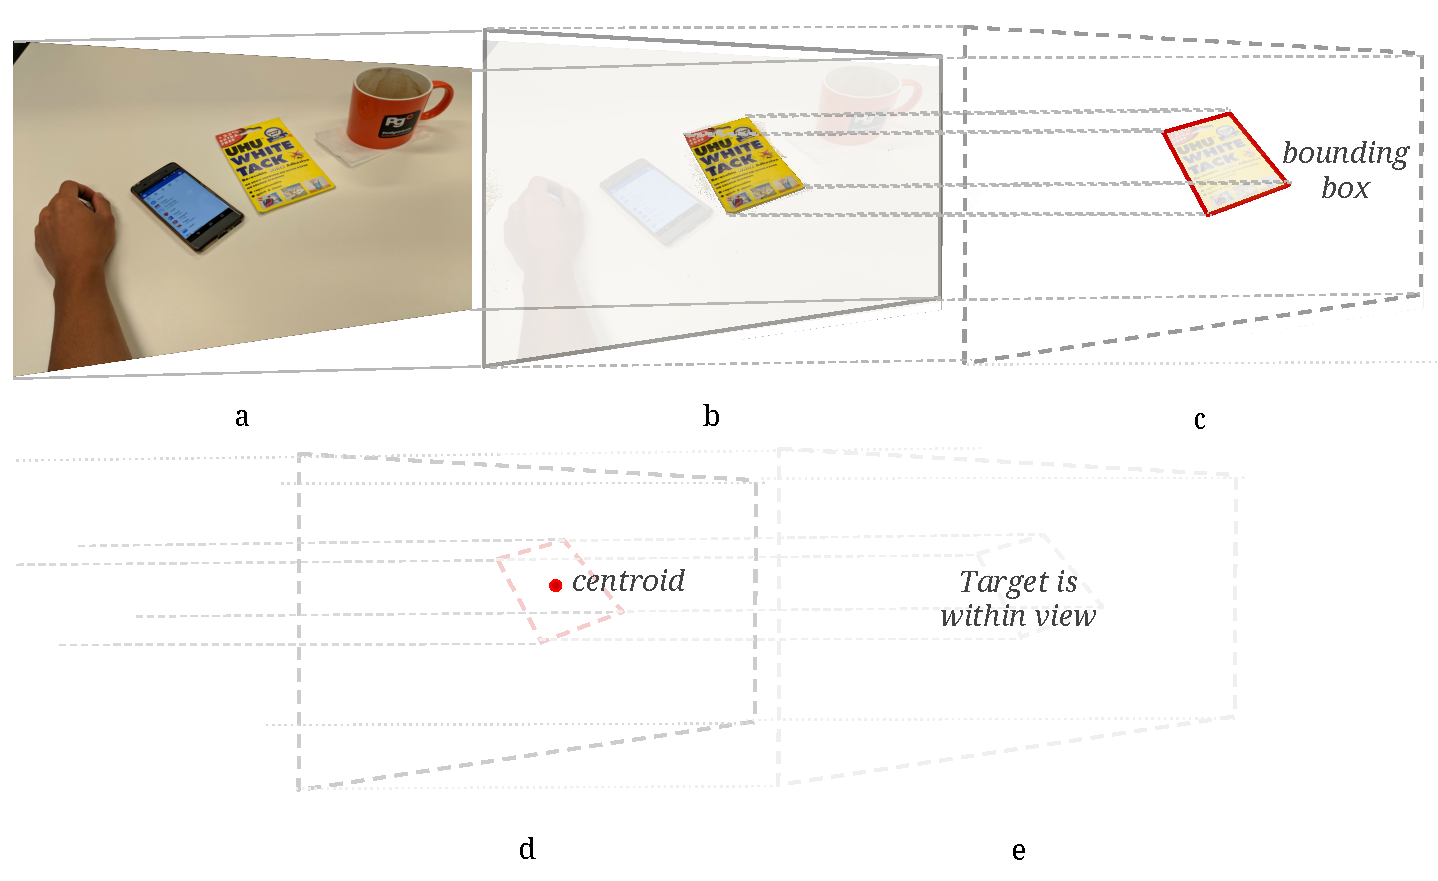
\includegraphics[width=\columnwidth]{figures/privilege-information-hierarchy-vertical}
%	\caption{Diminishing information: a) the raw visual capture; b) the target is cropped out but still with complete visual information of the target; c) only the bounding box of the target is exposed; d) only the centroid of the target is exposed; and e) only the binary presence, whether the target is within view or not, is exposed.}
%	\label{fig:privilege-levels}
%\end{figure}

%Thus, it is necessary to have \textit{visual information protection} in MR. %To provide \textit{user-originated} privacy protection, 
%We present an access control mechanism for raw data access with fine granularity through object-level abstractions. That is, we insert an \textit{intermediary} layer of protection that filters the visual information that is passed to third party applications. Figure~\ref{fig:privilege-levels} shows a cascading and diminishing visual information representation. Our approach releases information at the level shown in Fig.~\ref{fig:privilege-levels}.c, i.e. the bounding box coordinates of the objects within view, is exposed instead of the raw visual image capture.
%
%There have been a few works in the general space of AR/VR/MR that uses abstraction as a form of protection. However, to the best of our knowledge, this is the first demonstration of a generalized object-level abstraction as a form of access control for privacy protection.

\section{3D Privacy Problem}%{Theoretical Framework}
\label{sec:framework}

\begin{figure}[t!]
	\centering
	\vspace{-2mm}
	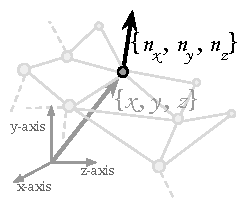
\includegraphics[width=0.4\columnwidth]{figures/3D_data_point_description}%,height=0.12\textheight
	\vspace{-4mm}
	\caption{An oriented point with position vector $\{x,y,z\}$ and normal vector $\{n_x, n_y, n_z\}$. {\small The x- and z-axis indicate the point's ground position while the y-axis indicates its elevation.}}
	\vspace{-2mm}
	\label{fig:3D-data-point}
\end{figure}

We formalize the definitions for our 3D privacy problem as well as the privacy and utility metrics in \S\ref{subsec:definition}, and the adversary model in \S\ref{subsec:threat}. But, before we proceed with the 3D spatial privacy problem, we first introduce 3D data representation.
% Please add the following required packages to your document preamble:
% \usepackage{booktabs}

\subsection{3D Data}\label{subsec:3d-data}
There are various ways that MR-capable devices capture and compute 3D spatial data but all would result in the creation of a 3D spatial map represented by a set of \textit{oriented points}. These are 3D points described by their xyz-position in space usually accompanied by a normal vector as shown in Fig. \ref{fig:3D-data-point}; thus, each oriented point can be represented by a 6-element array $\{x, y, z, n_x, n_y, n_z\}$. These are the minimum information necessary to capture the \textit{geometric} properties of 3D spaces. In the case where normal vectors are not readily available (such as the case for the point clouds produced by Google ARCore), an estimation is produced from the points themselves. Furthermore, in some occasions, point clouds may also be accompanied by \textit{photometric} information such as color, i.e. RGB, or lighting intensity. For this work, we will only be focusing on the use of geometric information and leverage them for 3D description for emulating adversarial inference.

\begin{figure*}[t]
	\centering
	\vspace{-2mm}
	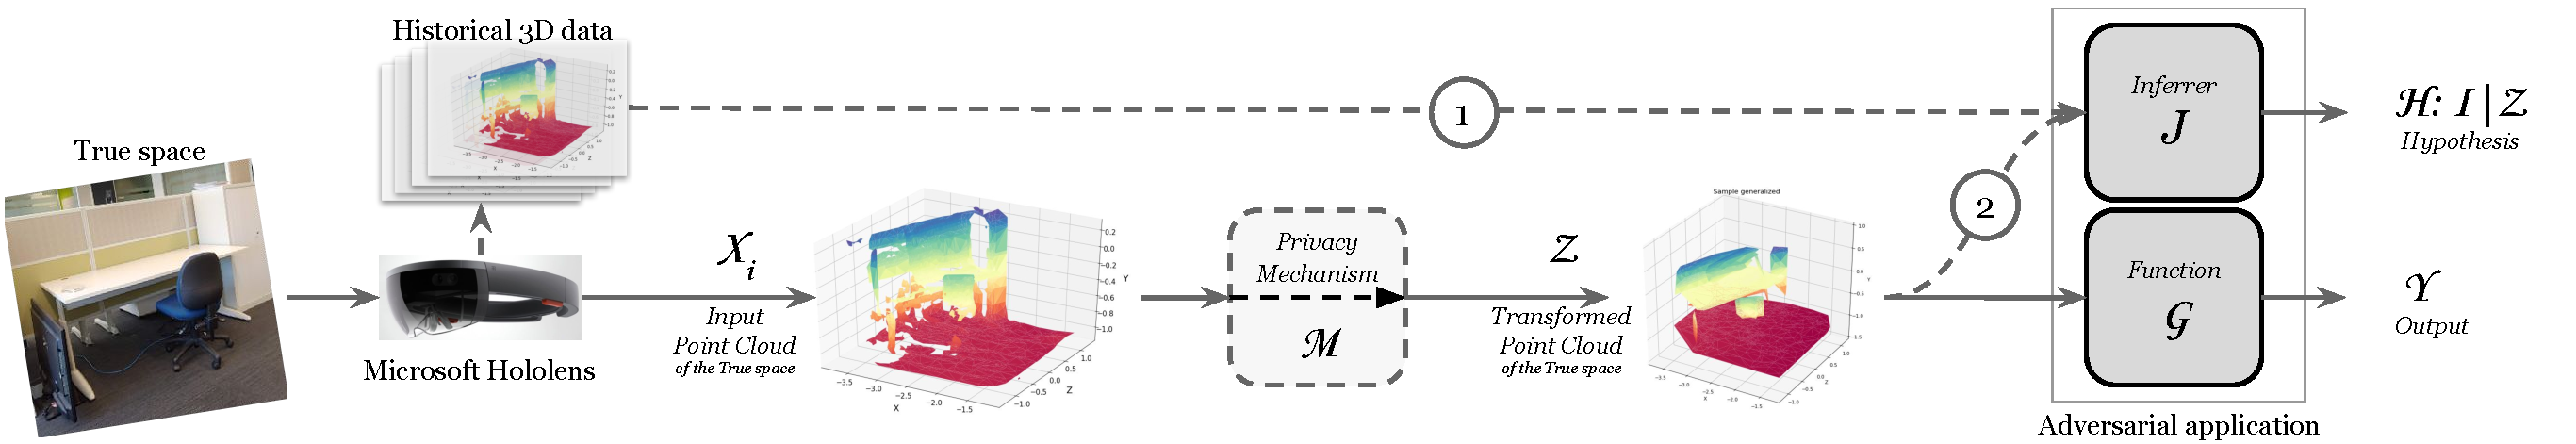
\includegraphics[width=0.95\textwidth]{figures/adversary-model-pipeline-v2.pdf}%,height=0.12\textheight
	\vspace{-2mm}
	\caption{Pipeline diagram of an MR adversary: {\small (1) adversarial inference \textit{modeling} or \textit{learning} from, say, historical 3D data (may be done off line), and (2) adversarial inference or \textit{matching} over released 3D data, say, during run time (More details in \S\ref{subsec:definition}, \S\ref{subsec:threat})}}
	\vspace{-2mm}
	\label{fig:adversary-model-pipeline}
\end{figure*}

\renewcommand{\arraystretch}{1.15}

\begin{table}[]
	\caption{Notation Map}
	\label{tab:notation-map}
	\vspace{-2mm}
	\centering
	\resizebox{0.75\columnwidth}{!}{
	\begin{tabular}{@{}cl@{}}
		\toprule
		\textbf{Notation} & \textbf{Description} \\ \midrule
		$X_i$ & raw representation of physical space labelled $i$ \\
		$F$ & Point-cloud extraction function            \\
		$v$ & $ \in R^3$, pose or reference view vector             \\
		$x_{i,v}$ & extracted point cloud of space $i$ given a pose $v$            \\
		$M$ & privacy-preserving mechanism             \\
		$z_{(i),v}$ & transformed point released by $M$            \\
		$G$ & intended functionality (i.e. MR app or service)             \\
		$y_{i,v}$ & output of the intended functionality $G$     \\ 
		$D_{Z;X}$ & difference of the transformed $Z$ from $X$  \\ 	
		$U(Z;X)$ & utility of the transformed $Z$ from $X$  \\
		$J$ & adversarial inferrer;  $J^!$ is the informed version  \\	
		$h$ & hypothesis of J about an unknown query space $i^*$  \\	
		$\Pi(Z;X)$ & privacy measure in terms of inference error  \\	\bottomrule
	\end{tabular}}
\end{table}

\subsection{Defining the 3D privacy problem}\label{subsec:definition}

To formalize the 3D problem, we define the following elements as shown in Fig. \ref{fig:adversary-model-pipeline}: the space represented by a point cloud $X$ identified by a label $i$; the privacy preserving mechanism $M$ that transforms $X$ to a privacy-preserved point cloud $Z$, i.e. $M : X \mapsto Z$; an intended functionality $G$ that produces an intended output $Y$, and from which we derive the utility function $U$; an adversarial inferrer $J$ that produces a hypothesis $H$ to reveal the identity of a given unknown space; and a privacy function $\Pi$. Table \ref{tab:notation-map} shows the notation map of the symbols used from this point onwards.

\emph{\textbf{Defining the input space.}} Let $X_i$ be the raw representation of space $i$ for any location in the real-world. A point-cloud extractor $F$ takes pose information vector $v \in R^3$ and releases a point cloud $x_{i,v}$ relative to that pose,
\begin{equation}
F : X_i,v \rightarrow x_{i,v},
\end{equation}
for any 3D space with location $i$ and a reference pose $v$.

Combining $x_{i,v}$ produces a complete point-cloud representation of space $X_i$, which we label as $\hat{X_i} = \bigcup_{v} x_{i,v}$ $\forall v$. An extension of this is that for any $v \in R^3$, we get a partial point-cloud representation $X_{i,v}$ of the true space. And that there exists a set of $v_s \subset V $ such that
\begin{equation}
	\hat{X}_{i,v_s} = \bigcup_{v \in v_s} x_{i,v}
	\label{eq:span-x}
\end{equation}
 spans $X_i$ or $\hat{X}_{i,v_s}=X_i$.

\emph{\textbf{Defining the abstraction.}} A privacy-preserving mechanism $M$ transforms any released point cloud $x_{i,v}$ to a privacy-preserving version $z_{(i),v}$,
\begin{equation}
M : x_{i,v}  \rightarrow z_{(i),v},
\end{equation}
where we denote the privacy-preservation of $i$ by ($i$) -- that is, the true $i$ of a released $z$ is not divulged or kept secret. Fig. \ref{fig:3D-privacy-problem} shows a simple visualization of the transformation that can occur. In this specific case, the normal vectors of the adjacent points are aligned to create a flat surface.

\begin{figure}[t!]
	\centering
	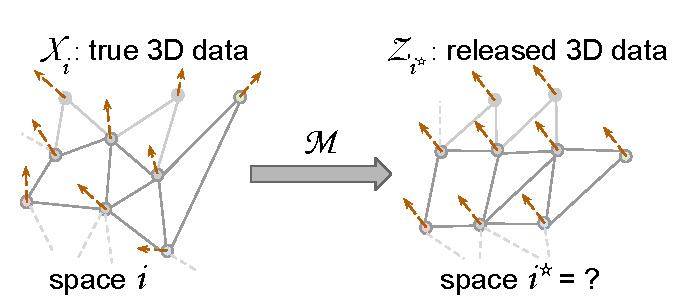
\includegraphics[width=0.7\columnwidth]{figures/3D_data_points}%,height=0.12\textheight
	\vspace{-2mm}
	\caption{\small{A privacy preserving mechanism $M$ converts (or generalizes) the raw point clouds $X$ to a \textit{potentially} privacy-preserving version $Z$ to \textit{hide} the identity ($i^* = ?$) of the space or location.}}
	\vspace{-2mm}
	\label{fig:3D-privacy-problem}
\end{figure}

Similar to the raw point-clouds $x_{i,v}$, combining the privacy-preserving point-cloud representations $z_{(i),v}$ produces
\begin{equation}
	\hat{Z}_{(i)} = \bigcup_{v} z_{(i),v}
	\label{eq:span-z}
\end{equation}
for all $v\in V$, or $Z_{(i)} = \bigcup_{v} z_{(i),v}$.

\emph{\textbf{Defining the intended functionality.}} An intended deterministic output $y_v$ produced by an intended application or functionality $G$ upon taking point clouds as the input, expressed as
\begin{equation}
	G :  x_{i,v},  { or }   z_{(i),v,} \rightarrow y_{(i),v}.
\end{equation}
For a given $G$, an effective mechanism $M$ aims to make the resulting outputs from the raw point cloud $x_{i,v}$ and its privacy-preserving version $z_{(i),v}$ similar, i.e. $y_{x_{i,v}} \simeq y_{z_{(i),v}}$, or their difference
\begin{equation}
	D_{Z;X} = |y_{x_{i,v}} - y_{z_{(i),v}} | \rightarrow 0
\end{equation}
small. Or in terms of a utility function $U$  which we intend to maximize (as close to 1 as possible if we assume that $D_{Z; X}\leq1$),
\begin{equation}
	U(Z; X) = 1 - D_{Z; X}
	\label{eq:utility}
\end{equation}
where $Z = M(X)$.

\emph{\textbf{Defining the adversarial inferrer.}} An inferrer $J$ produces a hypothesis $h : i^*=i$ about the true location $i$ of a given set of point clouds ${x_{i^*,v}}$ for any query space $i^*$ and $v$.
\begin{equation}
	J:{x_{i^*,v} for\ any\ i^*\ and\ v} \rightarrow h : i^*=i
\end{equation}
where the following probability holds
\begin{equation}
	P(h : i^*=i | {x_{i^*,v}} ) > P(h:i^*=i^o,\ for\ any\ i^o \neq i | {x_{i^*,v}} )
	\label{eq:bayesian}
\end{equation}

A modified or \textit{informed}\footnote{Informed of the mechanism $M$ that transforms raw point cloud $X$ to $Z$.} inferrer $J^!$ can also make a hypothesis for point cloud representations $z_{(i^*),v}$ for any $i^*$, and $v$,
\begin{equation}
	J^!:z_{(i^*),v}\ for\ any\ i^*,\ and\ v\ \rightarrow h : i^*=i,
\end{equation}
where, similarly, the following probability also holds
\begin{equation}
P(h : i^*=i | {z_{(i^*),v}} ) > P(h:i^*=i^o,\ for\ any\ i^o \neq i | {z_{(i^*),v}} )
\end{equation}

%\textcolor{red}{Replace error rate as the miss-classification rate.}

\emph{\textbf{The privacy-utility problem.}} Consequently, we can now pose the following \textit{privacy} function $\Pi$ in terms of the error rate of the inferrer,
\begin{equation}
	\Pi (Z;X) = \mean_ {iterations} \frac{|h: i_z \neq i_x|}{|\forall i|},
	\label{eq:privacy}
\end{equation}
which is simply the \textit{mean misclassification rate} of an inferrer $J$ about the query space $i_z$ whose true identity is $i_x$. A few works in the literature uses the same error-based metric for privacy \cite{Wagner:2018:TPM:3212709.3168389, shokri2011quantifying, narayanan2009deanonymizing}. A desired $M$ produces $Z$ that maximizes both the privacy $\Pi$ and the utility function $U$.

\emph{Privacy and utility metrics.} Now, we define the specific privacy and utility metrics for this work. For privacy, we use the same notion of a high error rate as high privacy; thus, the same metric defined by Eq. \ref{eq:privacy} holds. For utility, we use the same similarity definition defined by Eq. \ref{eq:utility} but define the specific components of the similarity function as,
\begin{equation}
U(Z;X) = \mean ( \alpha \cdot (1 - ||x - z||) + \beta \cdot (\vec{n_x} \cdot \vec{n_z}) )	
\end{equation}
where the first component is the 3D point similarity of the true/raw point $x$ from the transformed point $z$, the second component are their normal vector similarity, and $\alpha$ and $\beta$ are contribution weights where $\alpha, \beta \in \left[0,1\right]$ and $\alpha + \beta  = 1$. We set $\alpha, \beta = 0.5$. We also insert a subjective acceptability metric $\gamma \in \left[0,1\right]$ like so,
\begin{equation}
\begin{aligned}
U(Z;X) = \mean \left[ \alpha \cdot \left(1 - \frac{\ceil{||x - z||}_{\gamma}}{\gamma}\right) + \right. \hspace{7mm}\\
\left. \beta \cdot \left(\floor{\vec{n_x} \cdot \vec{n_z}}_{1-\gamma} - \frac{1-\gamma}{\gamma}\right) \right] .
\end{aligned}
\label{eq:utility-by-sim}
\end{equation}
$\gamma$ allows us to specify the level of error or deviation of the released (i.e. generalized) spaces from the true space -- any deviation beyond the set $\gamma$ results to a zero utility. The range of $U(X,Z) \in \left[0,1\right]$.

\subsection{Adversary Model}\label{subsec:threat}

Using the definitions in \S\ref{subsec:definition}, we can formalize the adversary models as previously shown in Fig. \ref{fig:adversary-model-pipeline}. We assume that the adversary is \textit{internal} and has \textit{prior knowledge} about the spaces which they can use as reference for building their inference model $J$. Prior knowledge can be made available through: (1) historical or publicly available 3D spatial data of the user spaces, (2) previously provided data by the user themselves or other users, or (3) from a colluding application or service that has access to raw or higher resolution 3D data.

Our adversarial inference is a two-step process as labelled in Fig. \ref{fig:adversary-model-pipeline}: (1) the creation of a reference description model or dictionary using the 3D descriptor algorithms (\S\ref{subsec:3D-description}) over the previously known spaces as reference, (2) and the inference of unknown spaces by \textit{matching} their 3D descriptors to that of the reference descriptors from step 1. The construction of the inference model is detailed in the next section. %The adversary model and these assumptions are further used to formulate the adversarial strategies described in the experiments in \S\ref{subsubsec:improved-matching}.

\section{3D Description and Inference}\label{sec:3d-space}
%Before we discuss the 3D spatial privacy problem, 
We, first, focus on the actual 3D data that we will be utilizing and its properties in \S\ref{subsec:3d-mr-data}. Then, discuss the different information extraction mechanisms used to describe the 3D space in \S\ref{subsec:3D-description} followed by the discussion on the inference algorithms in \S\ref{subsec:inference} which will be used for adversarial inference. Finally, we conclude this section with the validation in \S\ref{subsec:inference-validation} of the description and inference algorithms which shows that our chosen description algorithm are indeed translation- and rotation-invariant, and one of them, i.e. spin image description, performs very well even at very low point cloud resolutions.

\begin{figure}[t]
	\centering
	\begin{subfigure}[]{0.65\columnwidth}
		\centering
		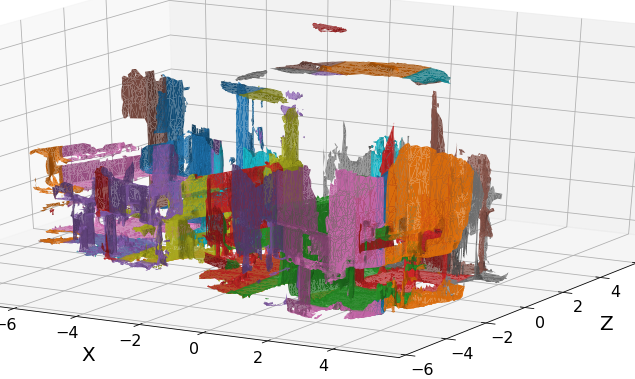
\includegraphics[width=\textwidth,height = 4cm]{figures/complete-point-cloud-3}
		\vspace{-3mm}
		\caption{\centering Complete captured raw point cloud:\newline different regions are differently colored}
		\label{fig:point-cloud-complete}
	\end{subfigure}
	\begin{subfigure}[]{0.34\columnwidth}
		\begin{subfigure}[]{\textwidth}
    		\centering
    		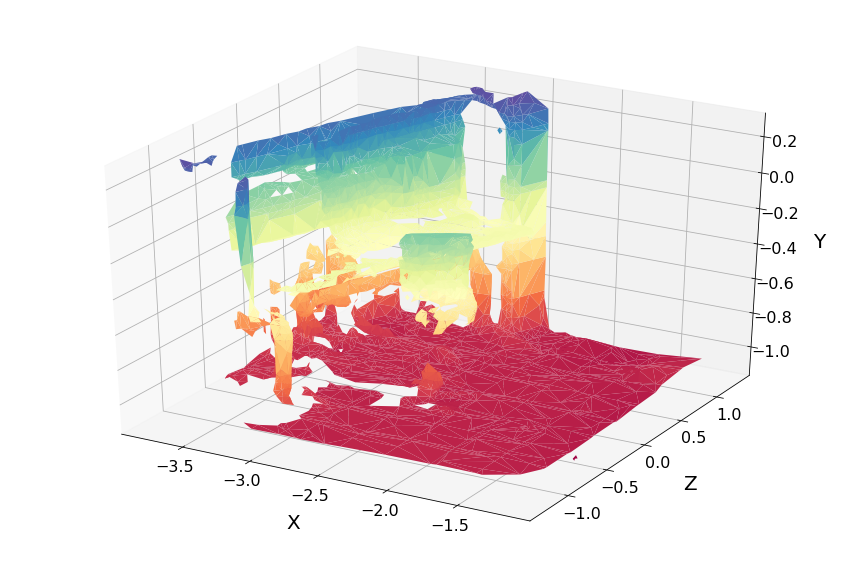
\includegraphics[width=\textwidth]{figures/sample-point-cloud-2}
    		\vspace{-3mm}
    		\caption{\small\centering Sample Region}
    		\label{fig:point-cloud-sample}
		\end{subfigure}
		\begin{subfigure}[]{\textwidth}
    		\centering
    		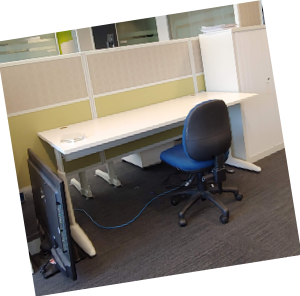
\includegraphics[width=0.5\textwidth]{figures/space-sample.png}
    		\vspace{0mm}
    		\caption{\small\centering Photo of the sample region}
    		\label{fig:photo-sample}
		\end{subfigure}
	\end{subfigure}
	\vspace{-2mm}
	\caption{Render of the gathered point cloud \small{(1 distance unit is roughly 1 meter in the real-world)}}
	\label{fig:point-cloud}
	\vspace {-2mm}
\end{figure}

\subsection{3D MR data}\label{subsec:3d-mr-data}

%\paragraph{Gathering sample data.}
We gathered real 3D point cloud data using the Microsoft Hololens in an office environment\footnote{There are numerous 3D point cloud datasets such as those listed in https://www.citygml.org/3dcities/ and http://cvgl.stanford.edu/resources.html among others, but we opted to use 3D data extracted from an actual MR device, i.e. a Microsoft Hololens, to demonstrate the leakage of actual spaces on which an MR device was used. Hololens hardware details at https://developer.microsoft.com/en-us/windows/mixed-reality/hololens\_hardware\_details}. The render of the gathered 3D space is shown in Fig. \ref{fig:point-cloud-complete}. We, then, sliced the complete point cloud about the xz-plane to create multiple spaces. Fig. \ref{fig:point-cloud-sample} shows a sample slice with a photo of the actual space shown in Fig. \ref{fig:photo-sample}. The resulting number of spaces after slicing is 38.

\renewcommand*{\thefootnote}{\fnsymbol{footnote}}
Fig. \ref{fig:point-cloud-properties} shows the properties of the gathered point cloud. The point population histogram is shown in Fig. \ref{fig:hist-point-count} and the average number of points per space is $1922$ points. The surface area histogram is also shown in Fig. \ref{fig:hist-surface-area} and the average surface area is $6.6$ $u^2$ (square-units; roughly equivalent to square-meters, $m^2$). The distribution of the inter-point distance (of points with a joining edge) is shown in Fig. \ref{fig:point-distance}. The minimum and maximum inter-point distance is 0.0025 u (1 distance unit is roughly 1 meter in the real-world) and 0.425 u, respectively, with a mean at  0.0734 u. The CDF of the spaces' normal vector similarity\footnote[2]{Computed using the average cosine similarity of a point's normal vector and of its neighbours: a value of 1 means very similar or normals are parallel, while a value of 0 means that their normal vectors are orthogonal} are shown in Fig. \ref{fig:cdf-normal-similarity} with plots for spherical and cubical surfaces also shown for comparison. A spherical surface (and any smooth surface with nil to minimal curvature changes or discontinuities) will have a fairly consistent normal vector similarity; thus, its values are generally near $1$ and will less likely have values $\leq 0.9$\footnote[3]{Only for a point neighbourhood size of $\leq 30$ used to compute the similarity values; larger neighbourhood size introduces more dissimilarity.}. On the other hand, a cubical surface will have edges which result in lower similarity values on points along and near those edges yet high values on points that lie on the same plane, i.e. cube face. As we can see, the majority of surfaces represented by the gathered point clouds have a normal vector similarity CDF more akin to a cubical surface than that of a spherical surface due to the edges that naturally occur on real physical spaces (i.e. edges from wall-to-floor, floor-to-table, and so on) which produces lower similarity values (i.e. green to darker green colored). There are, however, a few surfaces whose normal vector similarity CDF plots are more similar to that of the sphere's CDF (i.e. lighter green to yellow colored) with some difference from the presence of lower similarity values which is not present in the spherical CDF.
\renewcommand*{\thefootnote}{\arabic{footnote}}

\begin{figure}[t]
	\centering
	\begin{subfigure}[]{0.49\columnwidth}
		\centering
		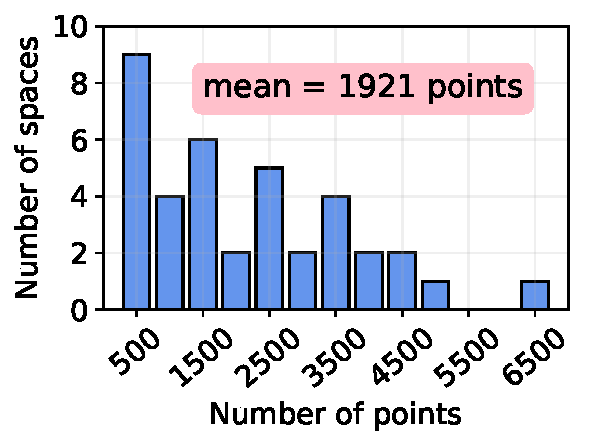
\includegraphics[width=\textwidth]{figures/plots/hist-point-count}
		\vspace{-5mm}
		\caption{Point population histogram}
		\label{fig:hist-point-count}
	\end{subfigure}
	\begin{subfigure}[]{0.49\columnwidth}
		\centering
		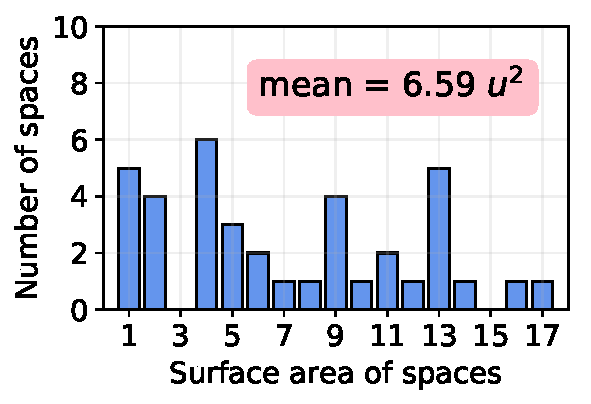
\includegraphics[width=\textwidth]{figures/plots/hist-surface-area}
		\vspace{-2mm}
		\caption{Surface area histogram}
		\label{fig:hist-surface-area}
	\end{subfigure}
	\vspace{2mm}
	\begin{subfigure}[]{\columnwidth}
		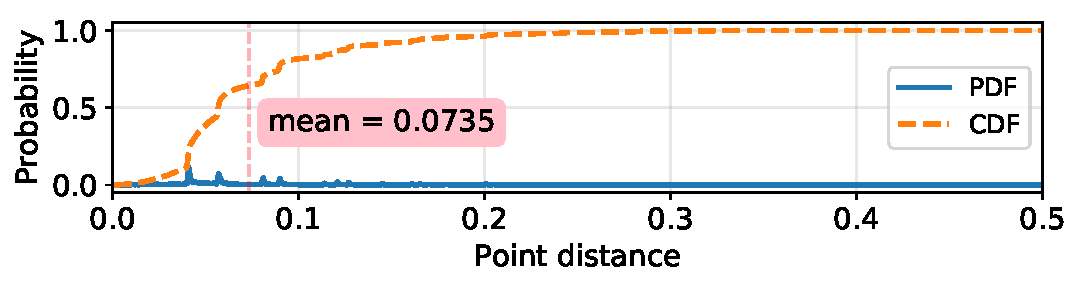
\includegraphics[width=0.925\textwidth]{figures/plots/point-distance}
		\vspace{-2mm}
		\caption{Inter-point distance distribution}
		\label{fig:point-distance}
	\end{subfigure}
	\begin{subfigure}[]{\columnwidth}
		\centering
		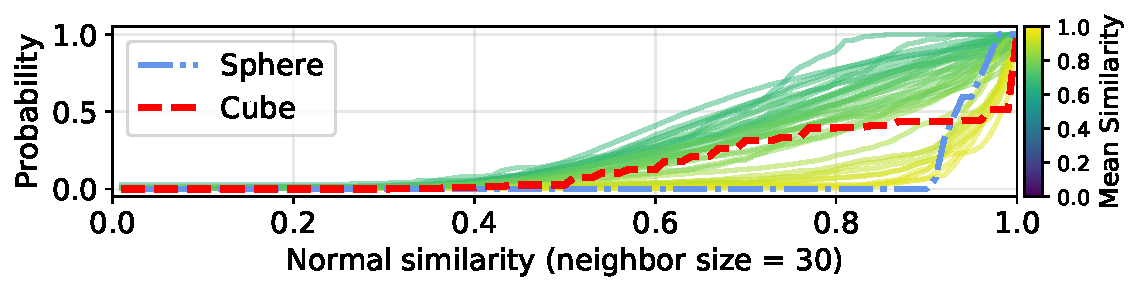
\includegraphics[width=\textwidth]{figures/plots/cdf-normal-similarity}
		\vspace{-5mm}
		\caption{Normal vector similarity CDF}
		\label{fig:cdf-normal-similarity}
	\end{subfigure}
	\begin{subfigure}[]{\columnwidth}
    	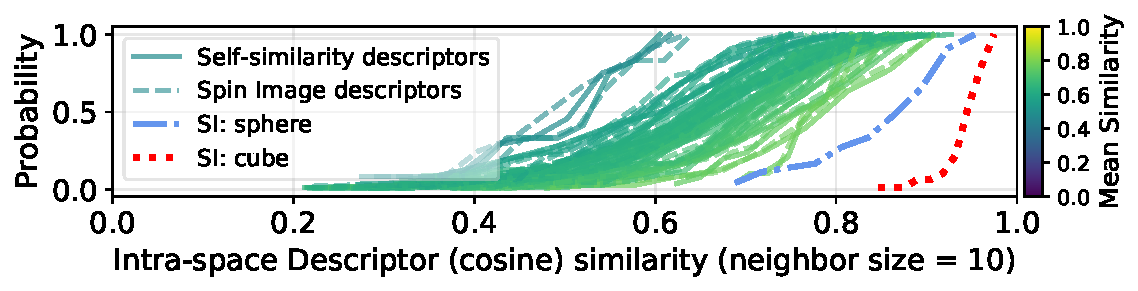
\includegraphics[width=\columnwidth]{figures/plots/descriptor-similarity.pdf}
    	\vspace{-4mm}
    	\caption{Descriptor similarity CDF}
    	\label{fig:descriptor-similarity}
	\end{subfigure}
	\vspace {-2mm}
	\caption{Properties of the point cloud dataset}
	\label{fig:point-cloud-properties}
	\vspace {-2mm}
\end{figure}

\subsection{Describing the 3D space}\label{subsec:3D-description}

%\textcolor{red}{Needs to be edited.}
These 3D spaces represented by point clouds can, then, be used by the adversary to train an inference model. Features that describes and discriminates among 3D spaces are usually used for inference modelling. There are enough features in 3D point clouds for it to be directly used as a 3D descriptor, albeit a crude one, and it won't be shift- and rotation-invariant by itself. These changes in space happen in real situations, such as when the reference point (x=0, y=0, z=0) changes for every MR session. Hence, inference models have to use invariant descriptors in order for an adversary to be resilient to these changes. 

To provide invariance, we utilize two existing 3D description algorithms: the curvature-reliant self-similarity descriptor \cite{huang2012point} (we'll use label SS), and the spin image descriptors \cite{johnson1998surface,johnson1999using} (we'll use SI). We choose these two for their relatively easier implementations in comparison to other 3D description algorithms such as the heat diffusion-based descriptors \cite{sun2009concise}. For a concise discussion and bench marking of different 3D description algorithms, we direct the reader to \cite{bronstein2010shrec}. For more details on our description algorithm implementation, please see Appendix \ref{apdx:descriptors}.%, we will briefly describe the two chosen 3D description algorithms and discuss their main difference. %Self-similarity descriptors

\renewcommand*{\thefootnote}{\fnsymbol{footnote}}

However, curvature-reliant descriptors, such as the SS descriptors, are very sensitive to point cloud variations, due to the curvature estimation, especially when normal vectors are also to be estimated. To counter this, we explored the use of non-curvature reliant 3D descriptors, i.e. the SI descriptors. SI descriptors are more dense compared to the SS descriptors due to the lack of a discriminative key point selection process. In addition, SI descriptors do not use any other metric or information other than the normal vector unlike the self-similarity approach which uses \textit{local curvature maxima} for key point selection. Thus, vanilla spin image computes the descriptor for every point in the point cloud which produces a dense descriptor space. For our SI implementation, we extract key points and descriptors from the subsampled space by factor of 3\footnote[7]{We choose sampling factor or resolution of 3 based on the performance shown in Fig.\ref{fig:performance} which shows that significant errors only appear at resolutions < 3.}.
\renewcommand*{\thefootnote}{\arabic{footnote}}Also, the spinning effect reduces the impact of variations within that spin which makes SI descriptors more robust to variations compared to SS descriptors. Furthermore, as we will describe in \S\ref{subsubsec:generalization}, surface generalization to planes removes curvatures which makes its use as a geometric description information impractical.

Figure \ref{fig:descriptor-similarity} shows the CDF of the descriptor similarity of the two algorithms. SS and SI descriptors extracted from the same space have a consistent and similar CDF plot as shown in the figure. The average number of descriptors extracted from our point cloud collection is $\sim 92$ for both SS and SI while the average similarity value are also both $\sim 0.65$. Descriptors extracted through either SS or SI have fair similarity; that is, most spaces will have a descriptor similarity of greater than 0.5 for the majority (i.e. > 50 \%) of their descriptors. We also include the descriptor similarities for our reference spherical and cubical spaces which, unsurprisingly, shows very high descriptor similarity values.
Validation of the inference performance of these descriptors are detailed in \S\ref{subsec:inference-validation}.

\subsection{Inferring the 3D space}\label{subsec:inference}

For the inference model to be used by our adversary, we built two types of \textit{inferrers}: (1) a \textit{baseline} 3D Bayesian inference model using the point clouds as features, (2) and a \textit{matching-based} inference model using the rotation-invariant descriptors.

\subsubsection{Bayesian Inference model using the point cloud}\label{subsubsec:bayesian}
To create the 3D Bayesian inference model, we create a 4-dimensional matrix $S_i\times X_{bins}\times Y_{bins}\times Z_{bins}$ with $S_i$ = the number of spaces, while the 3D bins are all pre-set, i.e. $X_{bins} = Y_{bins} = Z = _{bins}$ =  500 (250 for each +/- direction). We fill these bins using the number of points that fall within the defined $(\floor{x},\floor{y},\floor{z})$ and divide the total of every space to create a likelihood model $P(\textbf{X}_i | i)$ for every space $i$, where $\textbf{X}_i$ is the collection of point clouds, i.e. $\{(x,y,z)\}$, of space $i$. Now, a 3D inference model can be formulated as the maximization of the \textit{posterior probability} defined in Eq. \ref{eq:bayesian}, or as follows:
\begin{equation}
\max_{i}   P(h:i^*=i | {\textbf{X}_{(i^* = ?)}} )
\end{equation}
which aims to find a hypotheses $h:i^*=i$ about the query space $i^*$ that gives the maximum conditional probability of
\begin{equation}
P(h:i^*=i | {\textbf{X}_{(i^* = ?)}} ) =\frac{P(\textbf{X}_{i^*} | h: i^*=i) \times P(i)}{P(\textbf{X})}
\end{equation} given a set of points $\textbf{X}_{i^*}$.
The \textit{a priori} probabilities are set to $P(i) = \frac{1}{S_i}$ while the denominator $P(\textbf{X})$ (called the  marginal likelihood) is the total probability of the likelihood for all known  points, i.e. $\textbf{X}_i \forall i$, or specifically
\begin{equation}
P(\textbf{X}) =  \sum_{i} P(\textbf{X}_{i^*} | h: i^*=i) \cdot P(i).
\end{equation}
The resulting function to be maximized is as follows
\begin{equation}
\argmax_{i} \frac{P(\textbf{X}_{i^*} | h: i^*=i) \cdot P(i)}{\sum_{i} P(\textbf{X}_{i^*} | h: i^*=i) \cdot P(i)}.
\end{equation}

\subsubsection{Inference using the 3D descriptors}\label{subsubsec:feature-matching}

For the 3D descriptors, it is challenging to create a straightforward 3D inference model\footnote{Our self-similarity and spin image description implementation use have ($6\times 8 \times 6$) and 200 ($10 \times 20$) dimensions, respectively. If we are to approximate that each dimension will have 10 bins, it'll require $10^{288}$ or $10^{200}$ bins for every key point to be described approximately. Computational power is bound by the number of atoms in the universe which is estimated to be $10^{80}$ (maximum).} as we did previously in \S\ref{subsubsec:bayesian}. As a work around, we utilize the standard matching-based approach that is used over high-dimensional descriptors. This approach is rather \textit{deterministic} as opposed to the \textit{probabilistic} Bayesian inference model.

\paragraph{Defining the feature matching process.}
A matching function $\Upsilon$ maps two sets of features $f_a$ and $f_b$, of spaces $a$ and $b$, like so,
\begin{equation}
\Upsilon :f_a \mapsto f_b
\end{equation}

\begin{figure*}[t!]
 	\begin{subfigure}[]{0.235\textwidth}
		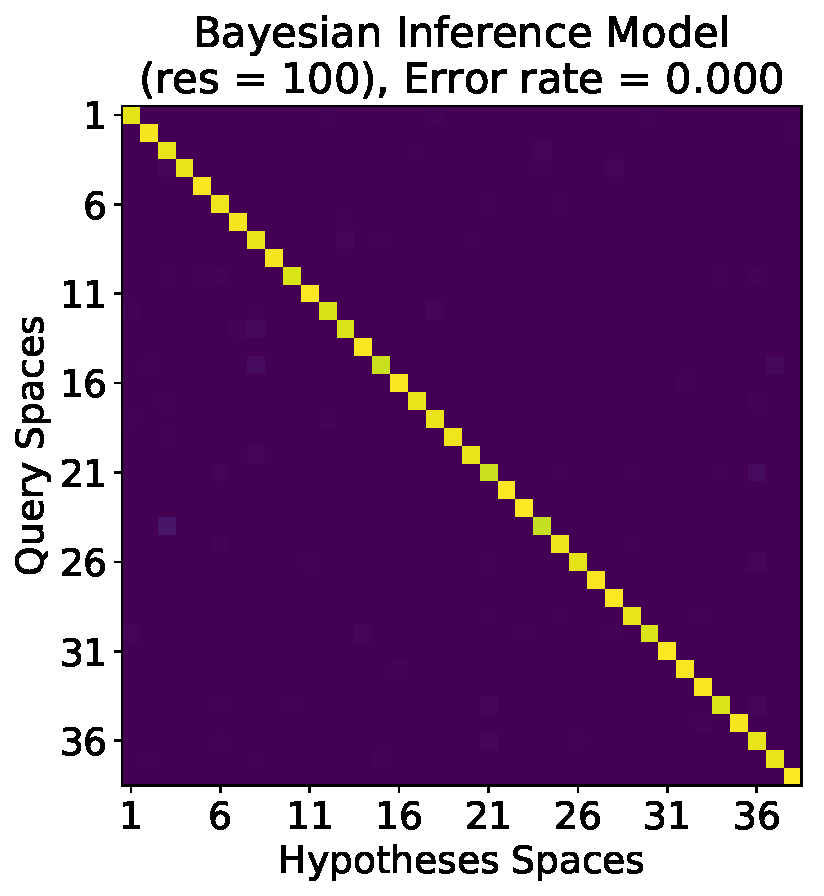
\includegraphics[width=\textwidth]{figures/plots/heatmap-b100}
		\caption{Bayesian (res = 100)}
			\label{fig:100-heatmap}
	\end{subfigure}
	\begin{subfigure}[]{0.235\textwidth}
		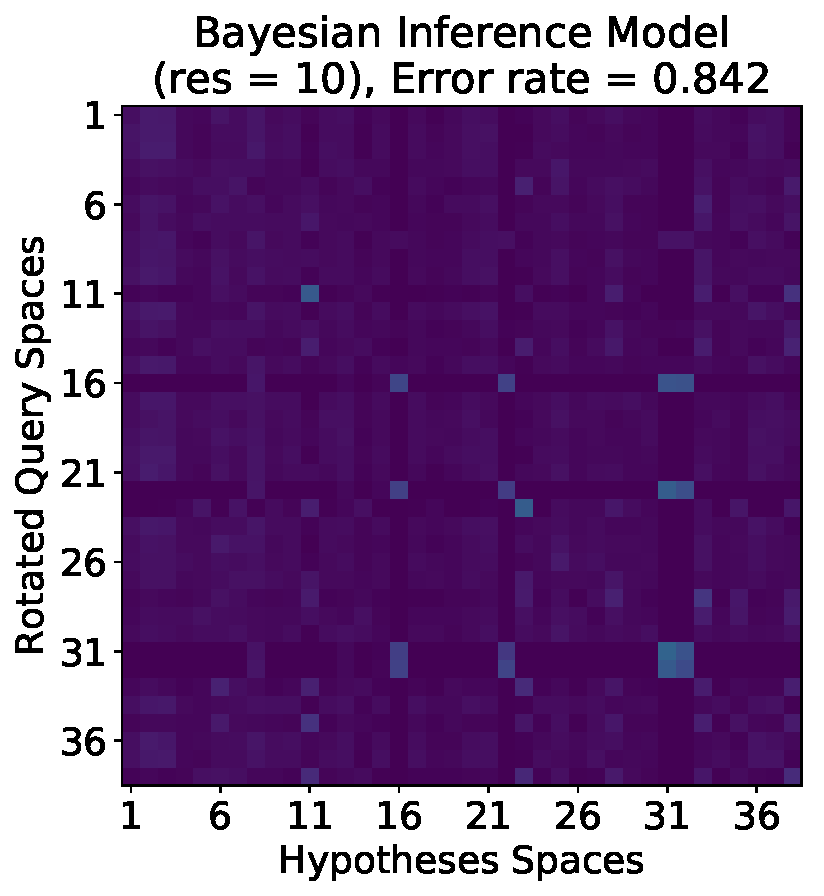
\includegraphics[width=\textwidth]{figures/plots/heatmap-b10}
		%\vspace{-10mm}
		\caption{Bayesian, rotated}
		\label{fig:heatmap-b}
	\end{subfigure}
	\begin{subfigure}[]{0.235\textwidth}
		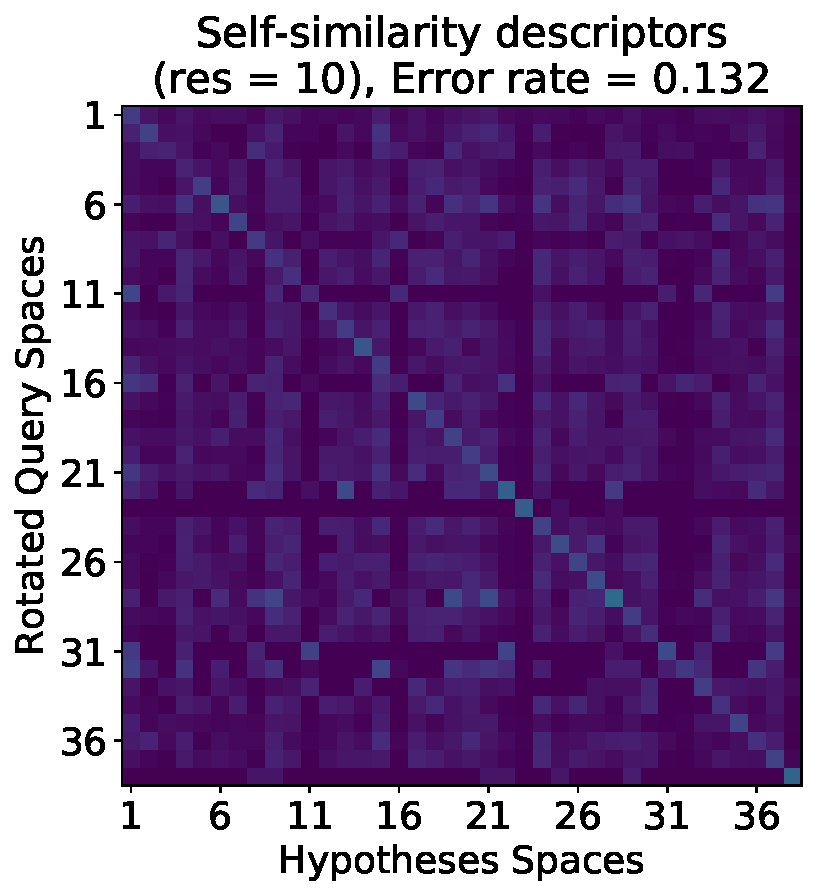
\includegraphics[width=\textwidth]{figures/plots/heatmap-ss10}
		%\vspace{-10mm}
		\caption{Self-similarity}
		\label{fig:heatmap-ss}
	\end{subfigure}
	\begin{subfigure}[]{0.235\textwidth}
		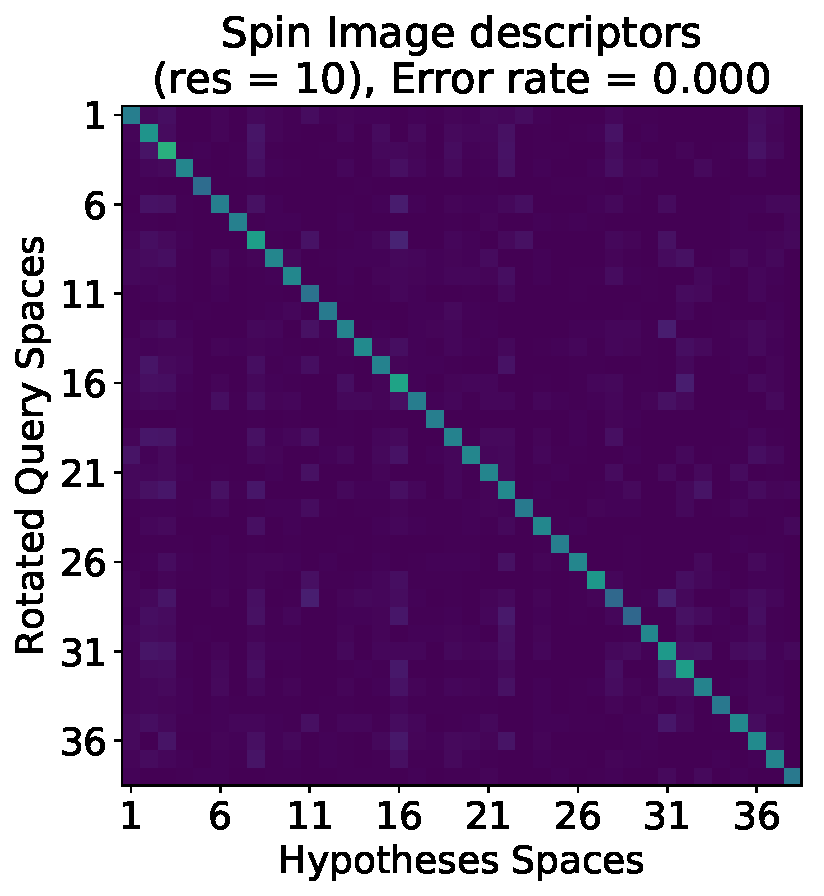
\includegraphics[width=\textwidth]{figures/plots/heatmap-si10}
		%\vspace{-10mm}
		\caption{Spin Images}
		\label{fig:heatmap-si}
	\end{subfigure}
	\begin{subfigure}[]{0.026\textwidth}
		\vspace{-7mm}
		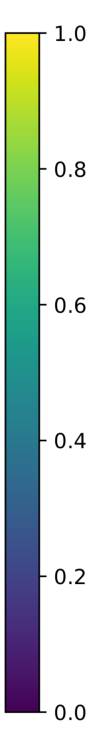
\includegraphics[width=\textwidth]{figures/plots/cbar}
		%\vspace{-10mm}
	\end{subfigure}
	\vspace{-2mm}
	\caption{Heatmaps of the different 3D description approaches}
	\label{fig:heatmaps}
\end{figure*}

To determine good matches, we use the descriptor Euclidean distance as a measure of their similarity. To \textit{accept} a match for a key point $x_{a,1}$ with feature $f_{a,1}$ of an unknown query space $a = i^*$, we get the \textit{nearest neighbor distance ratio} (NNDR) of the features like so,
\begin{equation}
\frac{||f_{a,1} - f_{b,1}||}{||f_{a,1} - f_{b,2}||} < threshold,
\label{eq:nndr}
\end{equation}
where descriptor $f_{b,1}$ of $x_{b,1}$ (i.e. key point $x_1$ of known space $b = i$) is the nearest neighbor of descriptor $f_{a,1}$ of $x_{a,1}$ (i.e. key point $x_1$ of unknown query space $a = i^*$) and $f_{b,2}$ is the second nearest neighbor, and see if the NNDR falls below a set threshold (e.g. 0.75 for the self-similarity, or 0.9 for the spin-image descriptors). Then, we maximum-normalize the distance of the accepted matches to make the maximum distance be 1. The mean of the distances is multiplied with a Bayesian-inspired weight,
\[
\frac{| \{f_{x_{i^*}} \mapsto f_{x_{i}}\} |}{|\{ f_{x_{i^*}}\}|} ,
\]
where $| \{f_{x_{i^*}} \mapsto f_{x_{i}}\} |$ is the number of matched descriptors of an unknown query space $x_{a = i^*}$ from one of the known reference spaces $x_{b = i}, i \in {\forall i}$, and $|\{ f_{x_{i^*}}\}|$ is the number of key points or descriptors extracted from the query space $x_{i^*}$. This allows us to create a hypothesis, i.e. $h: i^* = i$, also via argument-maximization as follows,
\begin{equation}
\argmax_{i}  \Big(1-\mean_{\{f_{x_{i^*}} \mapsto f_{x_{i}}\}} \{||f_{x_{i^*}} - f_{x_i}||\}\Big) \cdot \frac{| \{f_{x_{i^*}} \mapsto f_{x_{i}}\} |}{|\{ f_{x_{i^*}}\}|},
\label{eq:matching}
\end{equation}
where the first product term is the mean similarity (i.e. 1 -\textit{ mean difference}) while the second term is the Bayesian-inspired weight.

\subsection{Validating 3D Description and Inference}\label{subsec:inference-validation}
Before we proceed to the actual experiments demonstrating the spatial privacy leakage, we demonstrate here the preliminary validation that we conducted to check the effectiveness of the chosen description and inference approaches.

\paragraph{Validating the Bayesian Inference model.}

We created a Bayesian inference model as described in \S\ref{subsec:inference} using our gathered point cloud data (\S\ref{subsec:3d-mr-data}). To validate our inference model, we feed it the same data as queries. When complete versions of the set of points ${x_i}$ for each space $i$ is given as a query data, the inference model performs as shown in the heatmap/confusion matrix in Fig. \ref{fig:100-heatmap}. With complete data, the inferrer can give correct predictions with very high probability as shown by the solid yellow diagonal.

%Fig. \ref{fig:100-heatmap} shows the performance of an inference model with $r = 100$ -- i.e. having 100 points within a point cloud unit distance which is approximately one (1) meter in the real-world; thus, with $r = 100$, the smallest represented distance in the model is ~1 cm (per coordinate) or has a cube with volume ~1 cm$^3$.

We also investigated the effects of point resolution (or the sub- sampling factor) in our inference model. That is, we reduce the point resolution of the query spaces. Fig. \ref{fig:performance} shows the results of varying the resolution from $1 \leq res < 20$. For un-rotated query spaces, the baseline inference model only starts to have errors at resolutions $\leq 10$, while its error rate for rotated query spaces is $\geq 0.8$ for all resolutions. As we have indicated in \S\ref{subsec:3D-description}, the baseline inference model is not rotation-invariant and it is clearly observed here. For example, Fig. \ref{fig:heatmap-b} shows a heat-map for a lower resolution of res = 10 with rotated query spaces; we can not see a distinguishable diagonal to signify good inference performance.

\begin{figure}[t!]
	\vspace {-2mm}
	\centering
	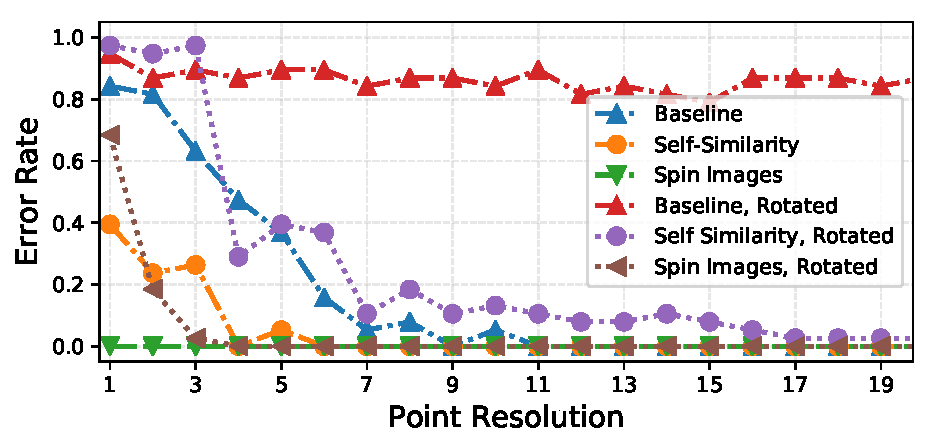
\includegraphics[width=\columnwidth]{figures/plots/2-validation}
	\vspace{-5mm}
	\caption{\small Performance of the different 3D description/inference for different resolutions ($1 \leq res \leq 20$)}
	\vspace{-2mm}
	\label{fig:performance}
\end{figure}

\paragraph{Validating the rotation-invariant descriptors.} Similarly, we also validate the performance of our rotation-invariant descriptors and show its performance in Fig. \ref{fig:performance}. With un-rotated query spaces, the self-similarity descriptors' maximum error rate is only 0.4, while the spin-image descriptors stays 0 even at the smallest resolution of 1. With rotated query spaces, errors increased for both but significant errors (i.e. $\geq 0.1$) only appear at res $\leq 3$ for the spin image descriptors, while errors for the self-similarity descriptors already appear even at higher resolutions of res $\leq 14$.

The excellent performance of the spin image descriptors can be better visualized with the heatmaps shown in Fig. \ref{fig:heatmaps} with res = 10. As can be observed, the spin images discriminates well as demonstrated by the clearer diagonal in Fig. \ref{fig:heatmap-si} as compared to \ref{fig:heatmap-ss}.
%We also extracted rotation-invariant descriptors from down-sampled reference point clouds and tested their matching performance with the descriptors extracted using the complete point clouds and those from a high resolution (i.e. res = 20). Fig. \ref{fig:performance-self} plots their matching performance. Indeed, the spin-image descriptors extracted from true points performs very well compared to the self-similarity descriptors and even with spin image descriptors extracted from a point cloud sub-sampled at res = 20, and even after rotations. 
Thus, in the succeeding experiments described in the next section (with results discussed in \S\ref{sec:discussion}), we will only be using spin image descriptors extracted from raw point clouds unless specified.

\section{Evaluation Setup}\label{sec:methodology}%Step 0: Privacy Leakage in 3D}\label{progress2}
For our evaluation, we use the same dataset that has been described in \ref{subsec:3d-mr-data}. We, first, introduce the spatial abstraction techniques in \S\ref{subsec:strategies}. Then, we describe the specific experimental setups in \S\ref{subsec:attack} which demonstrates adversarial inference to reveal 3D spaces which leads to spatial privacy leakage.

%\textcolor{red}{INCLUDE: (1) re-introduce the dataset, environment, etc. (2) the number of iterations, rotations, radii, (3) specific test cases , etc.}

%\subsection{Na\"ive Abstraction Strategies and Inference}\label{subsec:abstraction-strategy}
\subsection{3D information reduction strategies}\label{subsec:strategies}

%\textcolor{red}{Why generalize? True points and the generalized spaces.}
%
Directly releasing raw point clouds exposes all spatial information. To limit the amount of information released to applications, (1) plane generalizations and (2) partial releasing can be utilised to provide MR applications the least information necessary to deliver the desired functionality. 
%We present two major protection strategies, (1) partial spaces, and (2) generalizations, and their combinations as well as successive release of spatial data using these strategies.

\subsubsection{Plane fitting generalization}\label{subsubsec:generalization}

For the generalizations, we employed two techniques: the popular RAndom SAmple Consensus (RANSAC) plane fitting method \cite{fischler1981random}, and a simple locally-originated plane generalization (we use label LOCAL henceforth). Fig. \ref{fig:3D-privacy-problem} earlier shows what structurally occurs during plane-fitting generalization which can potentially preserve spatial privacy. Please see Appendix \ref{apdx:generalization} for the generalization pseudo-code (Alg. \ref{alg:ransac} \& \ref{alg:local-plane}). 

\begin{figure}[t!]
	\centering
	\vspace{-2mm}
	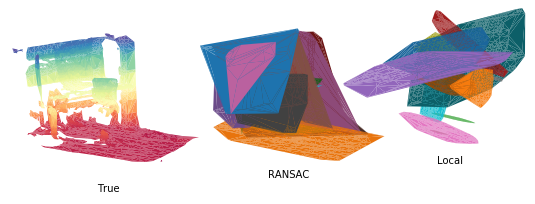
\includegraphics[width = \columnwidth]{figures/generalization_sample-8}
	\caption{Surface generalization, i.e. plane fitting, example: \small{(left) sample raw space, (center) RANSAC generalization, and (right) locally-originated generalization.}}
	\label{fig:generalization-example}
\end{figure}

\paragraph{\textbf{RANSAC.}}

For our implementation, we directly utilize the accompanying normal vector information to estimate the planes in the plane fitting process instead of computing or estimating them from the neighbours. Alg. \ref{alg:ransac} (in Appendix \ref{apdx:generalization}) shows the pseudo-code of our RANSAC implementation, while an example RANSAC spatial generalization is shown in Fig. \ref{fig:generalization-example}-center.

% SHOULD WE INCLUDE THE PLOT on NUMBER OF PLANES distribution?

\paragraph{\textbf{LOCAL.}}

On the other hand, the locally-originated plane generalization is an oversimplified version of RANSAC as can be seen in Alg. \ref{alg:local-plane}. We removed the point and plane test (Lines \ref{alg:point-test} and \ref{alg:plane-test} in Alg. \ref{alg:ransac}) which ensures that a point is a valid member of the candidate plane and that the candidate plane is the best, i.e. largest, among all candidate planes. This results in more inaccurate generalizations as we go further away from the initial test point from which the candidate plane originated. A sample localized generalization is also shown in Fig. \ref{fig:generalization-example}-right.

\subsubsection{Partial spaces}\label{subsubsec:partial-spaces}
In partial spaces, we only release \textit{segments} of the space with varying radius (in point cloud space units which is roughly equivalent to meters). This demonstrates the case when an MR application is provided with limited 3D spatial information only once, such as a specific surface, a plane or an anchor point. We apply this technique for both raw and \textit{generalized} point clouds.

%To demonstrate different 

\subsection{Attacking the strategies}\label{subsec:attack}

We use the information reduction techniques described in \S\ref{subsec:strategies} as abstraction strategies for privacy protection. First, we evaluated adversarial performance over \textit{one-time} released partial spaces as described in \S\ref{subsubsec:partial-spaces}. Then, we introduced more information by successively releasing partial spaces as described next.

%\subsubsection{Successive release of partial spaces}\label{subsubsec:successive-release}
\paragraph{Successive release of partial spaces.}\label{subsubsec:successive-release}
To demonstrate the case when users are moving around and their physical space is gradually revealed, we included an experimental setup that successively releases partial spaces. This also emulates the spanning described by Eqs. \ref{eq:span-x} \& \ref{eq:span-z}. Following the described abstraction strategies in \S\ref{subsubsec:generalization}, we have the following different 3D data setups for successively releasing:

\begin{enumerate}[leftmargin=*]
 \setlength{\parskip}{0.1mm}
  \setlength\itemsep{0em}
	\item partial spaces of true/raw points
	\item partial spaces from RANSAC generalized planes
	\item partial spaces from LOCAL generalized planes
\end{enumerate}

Also, we create 10 partial space iterations and further 5 random rotations for every case, and get the average metric values over these iterations.

\paragraph{Improving the matching-based adversarial inference.}\label{subsubsec:improved-matching}
As demonstrated during the validation in \S\ref{subsec:inference-validation} (Fig. \ref{fig:performance}), inference using spin image descriptors performs very well. However, significant variations can occur after generalizations. Specifically, points are forced to be co-planar resulting in it being translated from its original position, and their normals being forced to be the same as their neighbours. Thus, these variations can impact the inference.

To give our inference model additional resilience to these variations, we modify the matching described in \S\ref{subsec:inference} to incorporate two (entropy-reduction) techniques:

\textbf{Descriptor down sampling} \emph{(labelled Down-sampled)} - before matching, we interpolate, and down-sample the descriptors to effectively enlarge the descriptor bin sizes and reduce point variations within the enlarged bin.


\textbf{Query-biased Matching} \emph{(labelled Qry-Biased)} - to address the loss of points during release of partial spaces, we do an AND operation on the reference descriptors (which were extracted from raw points) with the non-zeros of the query descriptors, so that only the descriptor bins extracted from the available points of the partial query space contributes to the distance computation during feature matching (See Eqs. \ref{eq:nndr} \& \ref{eq:matching}).

\section{Results and Discussion}\label{sec:discussion}
We first show the inference performance for partial spaces that were provided only \textit{once} and where no further segments of the query spaces were revealed. As stated in Eq. \ref{eq:privacy}, we are using mean error rate as our privacy metric and uses this metric in succeeding plots and discussions. Afterwards, we successively release more segments of the spaces, which allows an adversary to collect more information and, thus, improve their performance (and decrease privacy). We also discuss the compactness of these inference models. %For the pre-abstraction validation of the description and inference algorithms, please refer to the results in \S\ref{subsec:inference-validation}.

\subsection{Inference of Partial spaces}\label{subsec:inference-partials}

\begin{figure}[t]
	\centering
	\vspace{-2mm}
	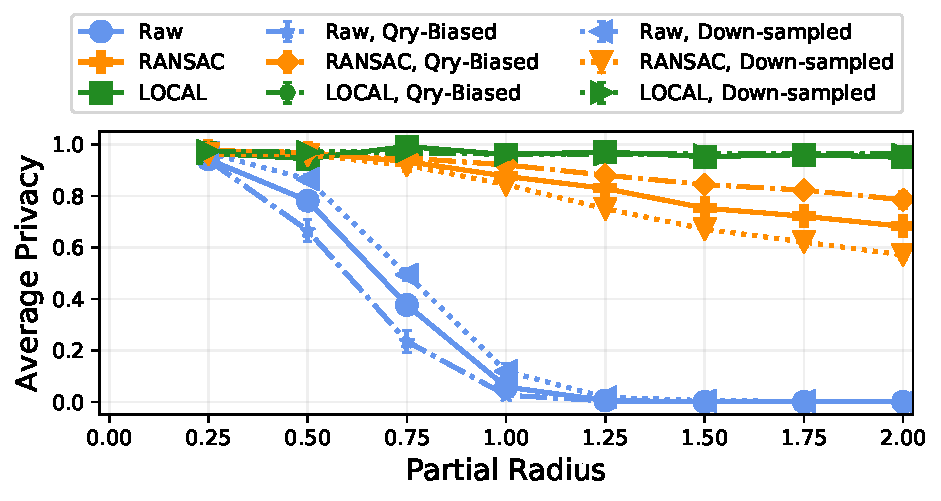
\includegraphics[width=\columnwidth]{figures/plots/partials-more-rotations}
	\caption{Inference over partial spaces with varying radii and different generalizations.}
	\label{fig:partial-all}
\end{figure}

%\begin{figure}[t]
%	\centering
%	\begin{subfigure}[]{0.49\columnwidth}
%		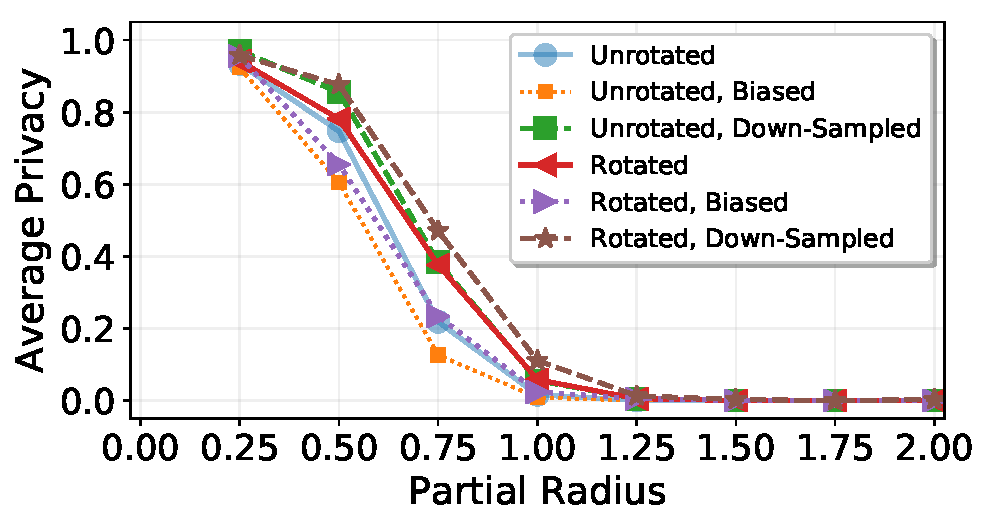
\includegraphics[width=0.92\textwidth]{figures/plots/2-partials-complete}
%   	\caption{True points}
%    	\label{fig:partial-complete-complete}
%	\end{subfigure}
%	\begin{subfigure}[]{0.49\columnwidth}
%		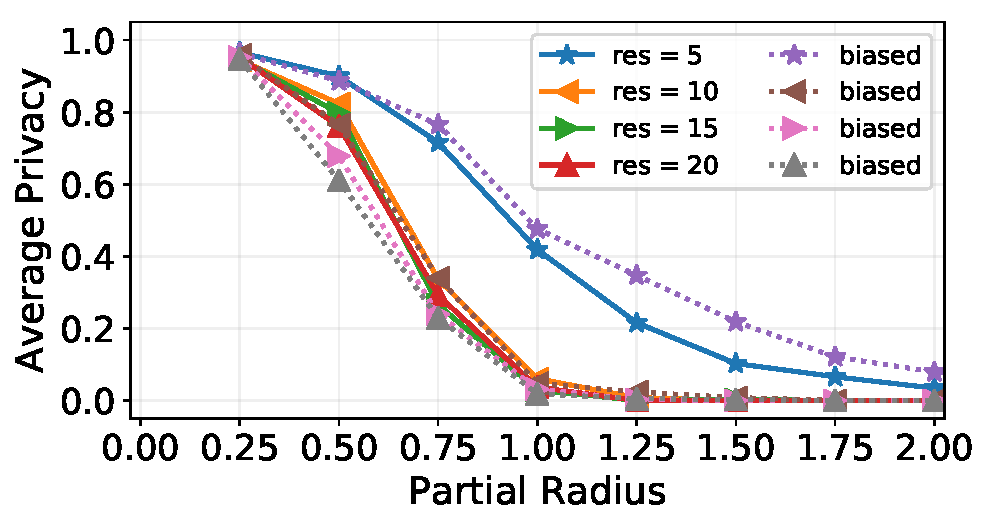
\includegraphics[width=0.92\textwidth]{figures/plots/2-partials-subsampled}
%    	\caption{Sub-sampled true points}
%    	\label{fig:partial-sub-complete}
%	\end{subfigure}
%	\begin{subfigure}[]{0.49\columnwidth}
%		\centering
%		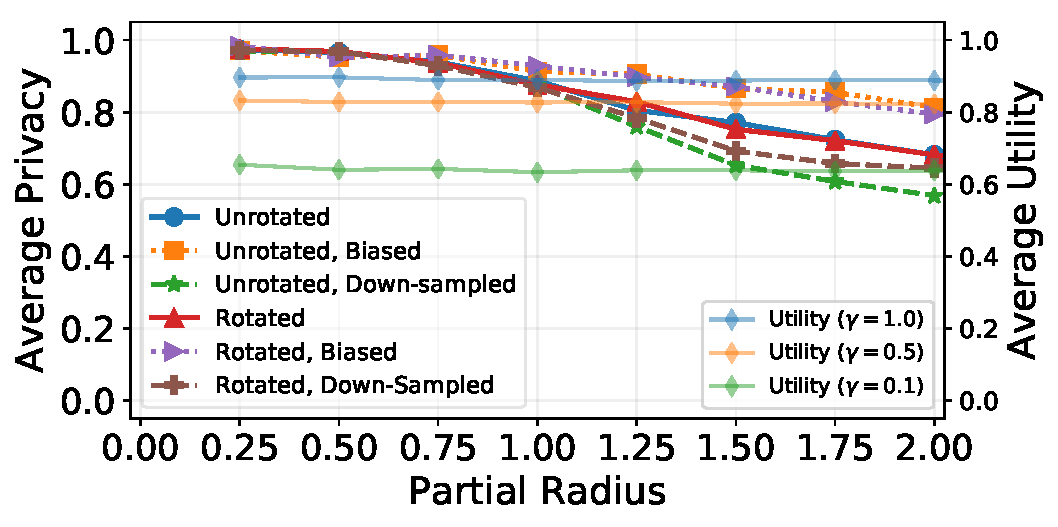
\includegraphics[width=\textwidth]{figures/plots/2-partials-ransac-with-utility}
%    	\caption{RANSAC generalized spaces}
%    	\label{fig:partials-ransac}
%	\end{subfigure}
%	\begin{subfigure}[]{0.49\columnwidth}
%		\centering
%		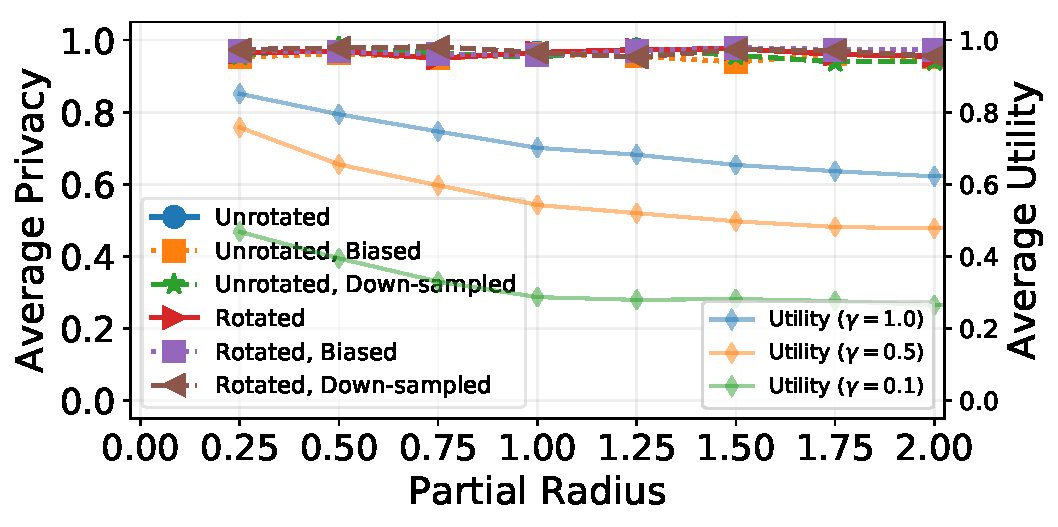
\includegraphics[width=\textwidth]{figures/plots/2-partials-localized-with-utility}
%    	\caption{Locally generalized spaces}
%    	\label{fig:partials-local}
%	\end{subfigure}
%	\caption{Inference over partial spaces with varying radii.}
%	\label{fig:partial-results}
%\end{figure}

\paragraph{Using raw spaces} Fig. \ref{fig:partial-all} shows the performance of our adversarial inference over partial spaces with raw points and of the two generalized cases. %We first evaluate the inference performance when using true and complete but partial spaces. Fig. \ref{fig:partial-complete-complete} shows the results for both un-rotated and rotated spaces as well as the performance improvement provided by the modified matching algorithms.
At radius $r = 0.25$, the average privacy is very high for all cases, but immediately drops below 0.8 at $r \geq 0.5$ for the raw-points case as well as its improved inference version by biased-matching. On the other hand, descriptor down-sampling does not improve the inference performance.

%On the other hand, Fig. \ref{fig:partial-sub-complete} shows the performance for sub-sampled point clouds and using biased-matching. For $res = 5$, the error rate is worse than that of the complete point clouds. This is expected as corroborated by the performance in Fig. \ref{fig:performance}. However, we can see that at $res \geq 10$, the inference performance now matches that of the complete point clouds in Fig. \ref{fig:partial-complete-complete}. %Also, the same improvement from biased-matching that we observed when using complete point clouds can also be observed for sub-sampled spaces of $res \geq 10$.

\paragraph{RANSAC generalized planes.} We applied the generalizations described in \S\ref{subsubsec:partial-spaces} and evaluated the inferrability of these partial spaces. Still in Fig. \ref{fig:partial-all}, it can be seen that the inference over partially revealed spaces that were generalized using the RANSAC algorithm is prevented with radius $r \leq 1.0$. Also, contrary to the raw-points case, the biased matching worsens the inference performance for RANSAC generalized spaces, while the down-sampling provides some improvement which brings the average privacy down by roughly 0.1. Thus, RANSAC generalizations are not effective protection strategies, especially for partially revealed spaces of radius $r \geq 1.0$. This should not come as a surprise, since the RANSAC algorithm will try to fit planes as close to the true/raw space (see Alg. \ref{alg:ransac} in the appendix).

\paragraph{Locally generalized planes.} On the other hand, locally-originated plane generalizations can prevent inference for this one-time partial release case. Regardless of the size of the revealed space, the average privacy stays above 0.9. And neither biased-matching nor down-sampling helps in the inference performance. In fact, contrary to RANSAC generalizations, locally-originated plane generalizations will maintain a high average privacy with larger revealed spaces because the LOCAL algorithm will only produce a generalized plane from a \textit{singular} reference point (see Alg. \ref{alg:local-plane} in the appendix) which may not even be from a true plane or have a normal vector consistent with its neighbours. This results in plane generalizations that are more likely to be very different from the surfaces of the true spaces.

\begin{figure}[t!]
	\centering
	\vspace{-2mm}
	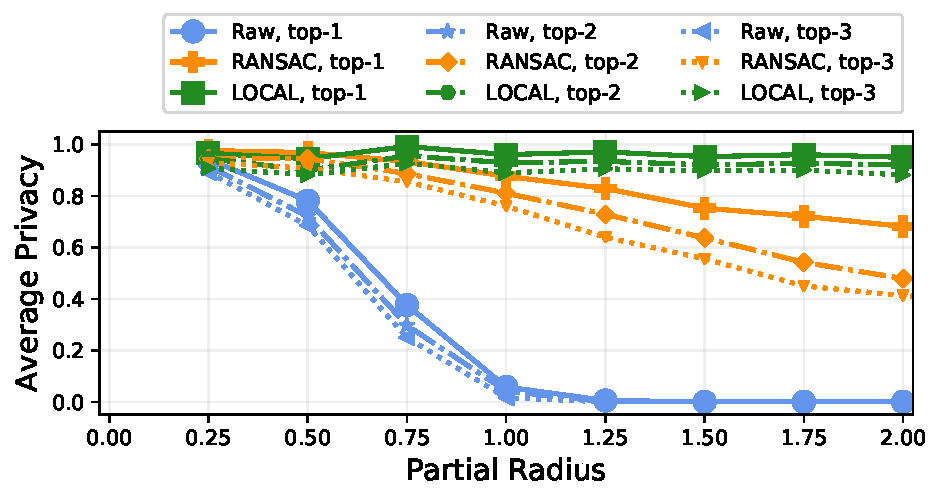
\includegraphics[width=\columnwidth]{figures/plots/2-partials-ranked.pdf}
	\caption{Inference over partial spaces with varying radii and generalizations but with additional top-\textit{n} results}
	\vspace{-2mm}
	\label{fig:partials-ranked}
\end{figure}

\paragraph{Top-n Results.}To show consistency of the adversarial inference, we also explored the next top ranked results to see whether the correct label, even if it does not have the highest inference score, is within the top-n scorers. Fig.\ref{fig:partials-ranked} shows the results when the correct label is within top-2 and top-3 scorers. As expected, there are improvements provided as we relax and check within the top-2 and 3 scored hypotheses. For the raw-points case, there was an average of 0.0141 decrease in average privacy over all radii which contributes to about 0.5 added hits over all spaces, when we count a hit if the correct label is within the top 2 scorers. For RANSAC, there was an average decrease of 0.0889 which contributes 3 more hits. Lastly, for the locally generalized case, there was an average decrease of 0.0317 which contributes about 1 added hit.

\subsection{Successive release}\label{subsec:inference-successive}
Following the partial spaces performance, it is tempting to say that we can maintain privacy by only releasing partial spaces of $r\leq 0.25$, but that is only for the single one-time release case. In this section, as described in \S\ref{subsubsec:successive-release}, we will now show the privacy or inference performance when we \textit{successively} release partial spaces. %we also evaluate the inference performance when successive partial spaces are released.


\paragraph{Raw-points spaces.} Fig. \ref{fig:successive-complete} shows the inference performance when partial query spaces are from the raw-points spaces. This is consistent with the results presented in Fig. \ref{fig:partial-all}. After a good number of releases, the space is slowly revealed; thus, the dropping average privacy. For $r = 0.25$, the average privacy only drops below 0.8 after 5 or more releases, while for the larger radii, $r = 0.75$, the average privacy quickly drops after the second release -- even starting at $\Pi_{Raw}< 0.8$.

\paragraph{RANSAC generalized planes.} For the successively released, RANSAC generalized partial spaces, as shown in Fig. \ref{fig:successive-ransac}, after 4 releases, the average privacy drops to $\Pi_{RANSAC}\leq 0.8$ for radius $r = 0.75$. Similar to the performance shown in Fig. \ref{fig:partial-all}, at higher radii, the average privacy for successive release eventually falls below $\le 0.6$ after a good number of releases. Specifically, for $r \geq 0.5$, the average privacy drops $\leq 0.6$ after about 14 releases.

Compared to the successively released partial spaces from raw points, the RANSAC generalization already contributes some errors to the released spaces. This reflects on the rather slow drop of the average privacy. Nonetheless, RANSAC generalization is still not a reliable protection approach from spatial inference especially when spaces are successively released. Eventually, no matter how small (i.e. $r \leq 0.25$) the released RANSAC-generalized partial space is, the inference performance improves after a few releases ultimately decreasing average privacy.

\paragraph{Local generalized planes.} Similar to the results in Fig. \ref{fig:partial-all}, the inference performance from successively released and locally generalized partial spaces, as shown in Fig. \ref{fig:successive-local-20}, presents error rates above 0.8 within 20 releases. In Fig. \ref{fig:successive-local-100}, we extend the number of releases to 96. Now, the average $\Pi_{LOCAL}$ do drop to $\leq 0.8$ for $r = 0.25$ ($r = 0.75$ approaches 0.8 at release 10) but eventually increases with more releases. Due to the high inaccuracy provided by localized generalizations, especially at larger partial spaces, more releases do not contribute to improved inference and only \textit{misleads} adversarial inference. Partially released planes with nearby originating points with different normals will produce planes within the same vicinity but of different orientations. This confuses the inferrer. Thus, if spatial privacy is a priority, localized generalizations can be used.

\begin{figure}[t!]
	\centering
	\begin{subfigure}[]{0.49\columnwidth}
		\centering
		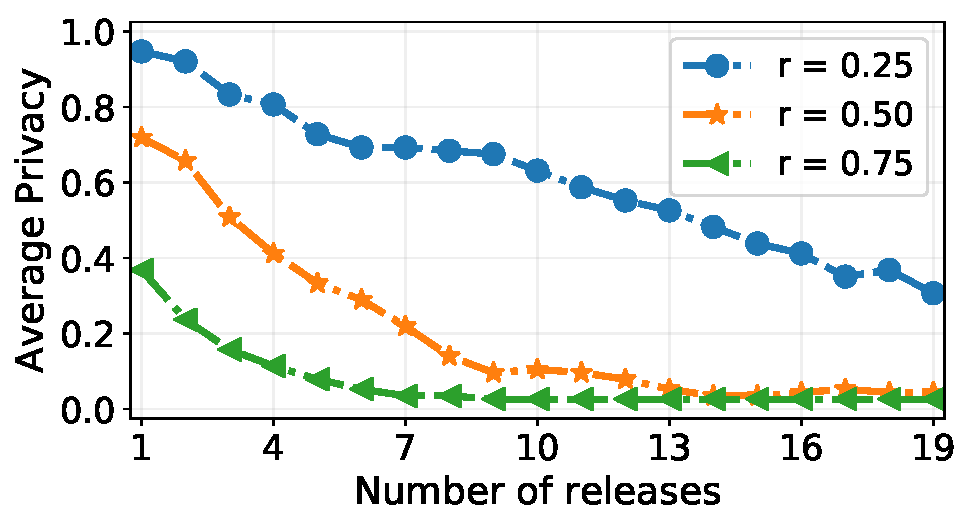
\includegraphics[width=\textwidth]{figures/plots/2-successive-complete-ranked}
	    \caption{Raw Points}
	\label{fig:successive-complete}
	\end{subfigure}
	\begin{subfigure}[]{0.49\columnwidth}
		\centering
		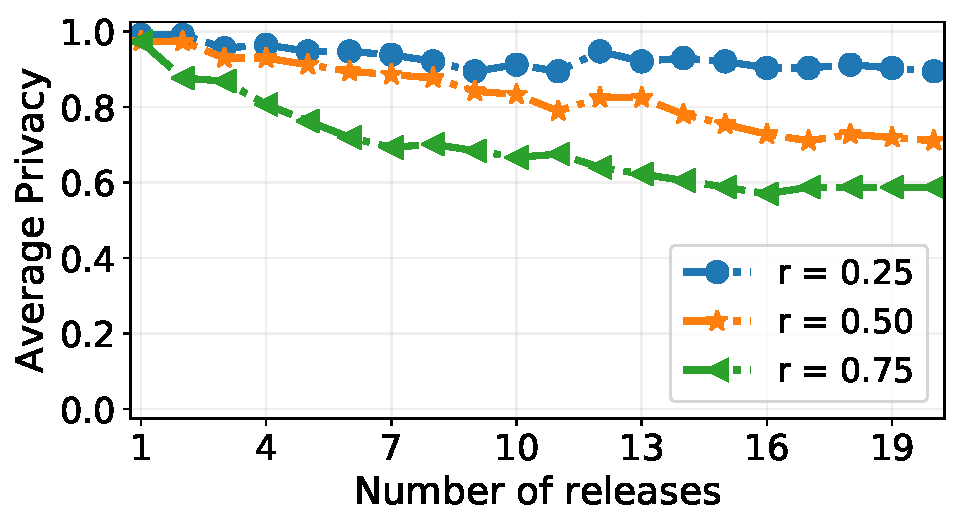
\includegraphics[width=\textwidth]{figures/plots/2-successive-ransac-ranked}
    	\caption{RANSAC generalized spaces}
    	\label{fig:successive-ransac}
	\end{subfigure}
	\begin{subfigure}[]{0.49\columnwidth}
		\centering
		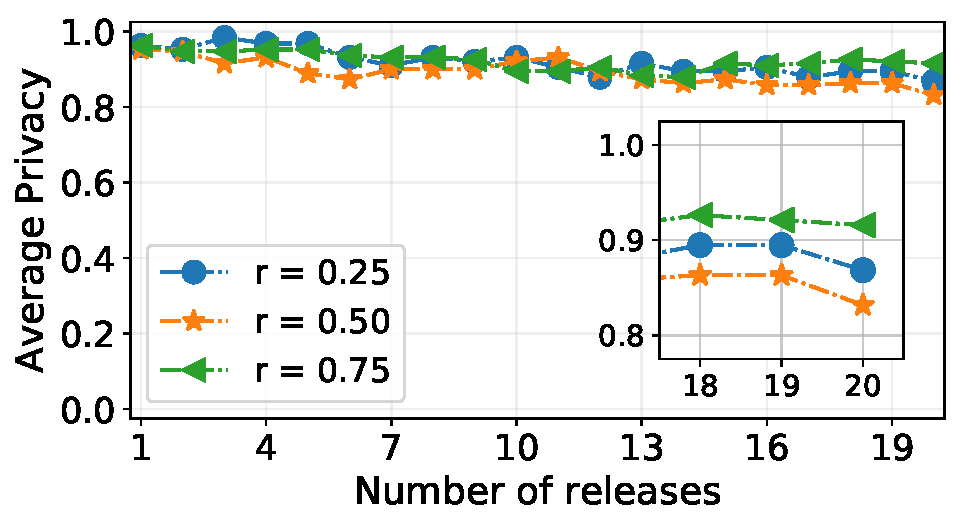
\includegraphics[width=\textwidth]{figures/plots/2-successive-local-ranked}
		\caption{LOCAL generalized spaces}
		\label{fig:successive-local-20}
	\end{subfigure}
	\begin{subfigure}[]{0.49\columnwidth}
		\centering
		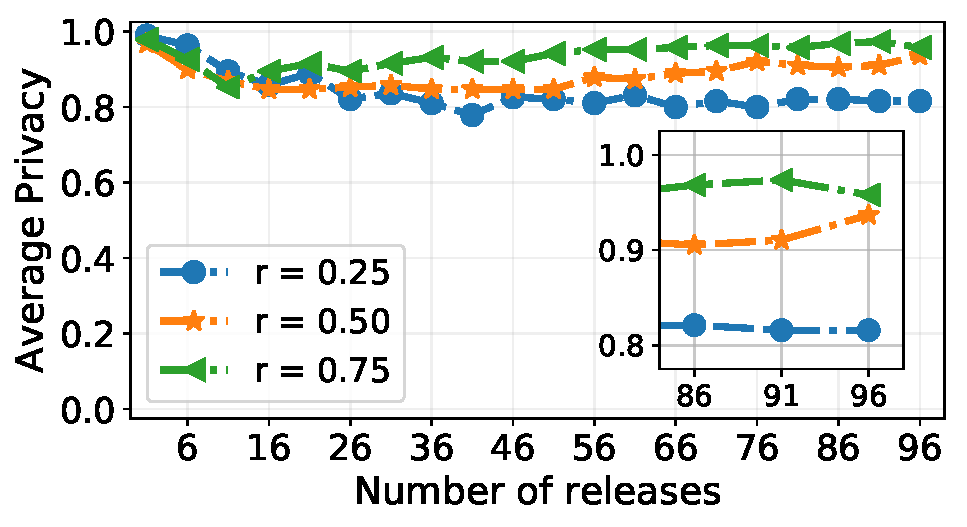
\includegraphics[width=\textwidth]{figures/plots/2-successive-local-extended-ranked}
    	\caption{\centering LOCAL generalized extended}
		\label{fig:successive-local-100}
	\end{subfigure}
	\caption{Inference over \textit{successively} released partial spaces.}
	\label{fig:partial-results}
	\vspace{-2mm}
\end{figure}

\emph{\textbf{Takeaway.}} \textit{The privacy based on the type of released space is as follows: $\Pi_{Raw} < \Pi_{RANSAC} < \Pi_{LOCAL}$. Also, for large enough spaces (i.e. r > 0.25), RANSAC still cannot provide adequate privacy especially in realistic successive releasing.}

\subsection{Inference trends with spatial properties}
%textcolor{red}{Focuses on the relationship between the properties of the spaces or descriptors with error rate}

\begin{figure}
	\centering
	\begin{subfigure}[]{0.62\columnwidth}
		\centering
		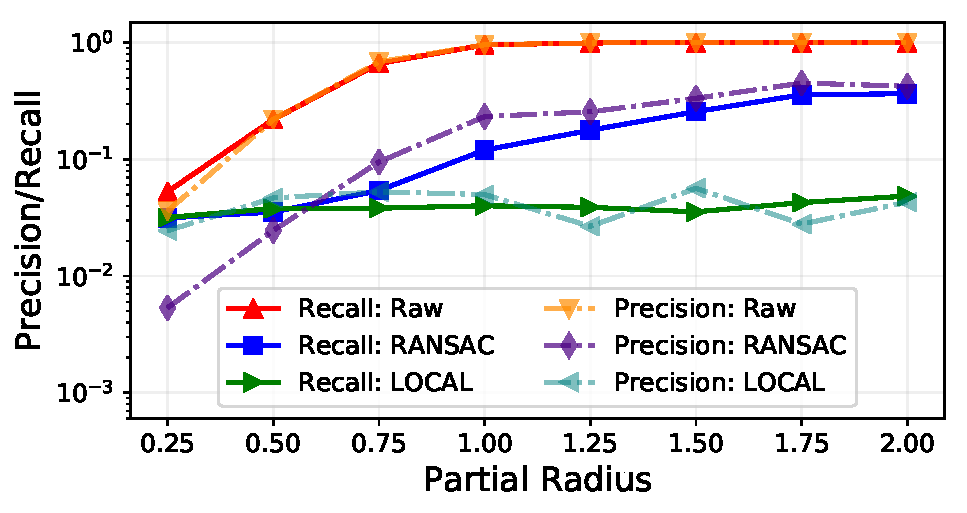
\includegraphics[width=\textwidth]{figures/plots/precision-recall-vs-radius.pdf}
    	\caption{\centering Precision and recall vs radius}
		\label{fig:precison-recall-radius}
	\end{subfigure}
	\begin{subfigure}[]{0.37\columnwidth}
		\centering
		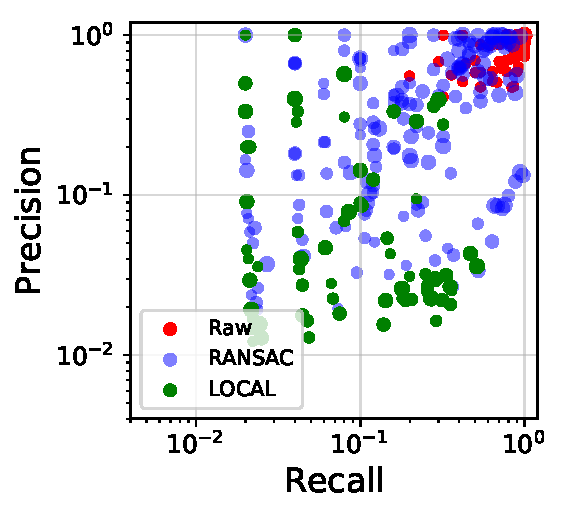
\includegraphics[width=\textwidth]{figures/plots/precision-vs-recall}
    	\caption{\centering Precision vs recall}
		\label{fig:precison-vs-radius}
	\end{subfigure}
	\caption{Precision and recall over partial spaces}
	\vspace{-2mm}
	\label{fig:performance-analysis}
\end{figure}

\paragraph{Precision and Recall.} We also checked the precision and recall as an inference performance metric. These values were checked for every space as well as the impacts of spatial properties on inference and/or privacy. Fig. \ref{fig:precison-recall-radius} shows the average precision and recall of our adversarial inferrer as we vary the radius of partial spaces. As expected, for raw-points spaces and RANSAC-generalized, precision and recall increases as the radius increases. On the other hand, locally-generalized precision and recall stays low, $<0.1$, and only ever so slightly increases -- from $0.032$ to $0.048$ for recall, and from $0.024$ to $0.043$ for precision -- but not consistently (as we  can see with the dips in $r = 1.25$ \& $1.75$).

Fig. \ref{fig:precison-vs-radius} shows the scatter plot of the precision and recall values for all spaces and iterations (averaged in Fig. \ref{fig:precison-recall-radius}) with the radius (relatively) depicted by the size of the circle. We can see that the values for the raw-points spaces crowd on the upper right quadrant, i.e. high precision and recall area, while that of RANSAC generalized spaces is slightly more scattered but also crowds on the upper right quadrant. For the locally-generalized spaces, most of the green circles reside on the lower half which means that recall is spread from low to mid-high but precision values are mostly very low.

Despite the bad performance of our adversarial inferrer, looking more closely in to the spaces reveals some consistency. Table \ref{tab:top-10} looks in to the top 10 spaces in terms of \textit{number of false positives}, \textit{precision}, \textit{recall}, and \textit{least errors/privacy}. We list the top 10 spaces for raw points, RANSAC generalized, and locally generalized. We, then, compared the list of top 10 spaces with least errors with the top 10 of the other performance metrics. We encircled spaces belonging to top 10 in terms of precision and put a star on spaces belonging to the top 10 in terms of their false positives. Recall and lesser errors have high correlation and treat them similarly (and no longer compare them). We also included the average number of planes of the top spaces in each category.

% Please add the following required packages to your document preamble:
% \usepackage{multirow}
\begin{table}[t]
\caption{Top 10 spaces in terms of \textit{aggregated} (all radii, rotations, and iterations) number of false positives, precision, recall, and less errors/privacy. We also show the average number of planes of these top spaces per category. \small{(Note: Spaces are arranged according to the space label and \textit{not} according to their metric values.)}}
\resizebox{0.98\columnwidth}{!}{
%
%\begin{tabular}{llllllllllll}
%\hline
%\multirow{3}{*}{\begin{tabular}[c]{@{}l@{}}False\\ Positives\end{tabular}} & %\textbf{C} & 4 & 5  & 7  & 9  & 10 & 24 & 26 & 29 & 30 & 34 \\ \cline{2-12} 
%                                                                           & \textbf{R} & 5 & 7  & 9  & 18 & 22 & 23 & 28 & 30 & 34 & 35 \\ \cline{2-12} 
%                                                                           & \textbf{L} & 5 & 10 & 12 & 18 & 20 & 23 & 26 & 28 & 34 & 35 \\ \hline
%\multirow{3}{*}{Precision}                                                 & \textbf{C} & 4 & 5  & 7  & 9  & 10 & 24 & 26 & 29 & 30 & 34 \\ \cline{2-12} 
                                                                           %& \textbf{R} & 5 & 7  & 9  & 18 & 20 & 24 & 26 & 29 & 30 & 34 \\ \cline{2-12} 
                                                                           %& \textbf{L} & 2 & 8  & 11 & 16 & 21 & 22 & 25 & 31 & 33 & 38 \\ \hline
%\multirow{3}{*}{Recall}                                                    & \textbf{C} & 8 & 11 & 16 & 22 & 23 & 31 & 32 & 33 & 35 & 38 \\ \cline{2-12} 
 %                                                                          & \textbf{R} & 4 & 5  & 7  & 13 & 18 & 24 & 26 & 30 & 31 & 33 \\ \cline{2-12} 
  %                                                                         & \textbf{L} & 1 & 2  & 4  & 8  & 11 & 13 & 15 & 16 & 31 & 38 \\ \hline
%\multirow{3}{*}{\begin{tabular}[c]{@{}l@{}}Least\\ Errors\end{tabular}}    & %\textbf{C} & 8 & 11 & 16 & 22 & 23 & 31 & 32 & 33 & 35 & 38 \\ \cline{2-12} 
 %                                                                          & \textbf{R} & 4 & 5  & 7  & 13 & 18 & 24 & 26 & 30 & 31 & 33 \\ \cline{2-12} 
                                        %                                   & %\textbf{L} & 2 & 4  & 8  & 11 & 13 & 15 & 16 & 27 & 31 & 38 \\ \hline
%\end{tabular}\\
\begin{tabular}{llllllllllllc}
\hline
&&&&&&&&&&&&{Ave. Planes}\\
\hline
\multirow{3}{*}{\begin{tabular}[c]{@{}l@{}}False\\ Positives\end{tabular}} & \textbf{Raw} & 1 & 8  & 11 & 16 & 17 & 25 & 27 & 31 & 33 & 38 &\textbf{4.21} \\ \cline{2-13} 
                                                                           & \textbf{RANSAC} & 2 & 8  & 13 & 15 & 16 & 27 & 31 & 33 & 36 & 38 & \textbf{4.38}\\ \cline{2-13} 
                                                                           & \textbf{LOCAL} & 1 & 2  & 4  & 8  & 13 & 15 & 16 & 27 & 31 & 38 & \textbf{6.11}\\ \hline
\multirow{3}{*}{Precision}                                                 & \textbf{RAW} & 4 & 5  & 7  & 9  & 10 & 24 & 26 & 29 & 30 & 34 & \textbf{14.44}\\ \cline{2-13} 
                                                                           & \textbf{RANSAC} & 5 & 7  & 9  & 18 & 20 & 24 & 26 & 29 & 30 & 34 & \textbf{13.77}\\ \cline{2-13} 
                                                                           & \textbf{LOCAL} & 2 & 8  & 11 & 16 & 21 & 22 & 25 & 31 & 33 & 38 & \textbf{2.3}\\ \hline
\multirow{3}{*}{Recall}                                                    & \textbf{Raw} & 8 & 11 & 16 & 22 & 23 & 31 & 32 & 33 & 35 & 38 & \textbf{3.21}\\ \cline{2-13} 
                                                                           & \textbf{RANSAC} & 4 & 5  & 7  & 13 & 18 & 24 & 26 & 30 & 31 & 33 &\textbf{11.59}\\ \cline{2-13} 
                                                                           & \textbf{LOCAL} & 1 & 2  & 4  & 8  & 11 & 13 & 15 & 16 & 31 & 38 & \textbf{5.41}\\ \hline
\midrule
\multirow{3}{*}{\begin{tabular}[c]{@{}l@{}}Least\\ Errors or \\ Privacy\end{tabular}}    & \textbf{Raw} & 1* & 11* & 16* & 22 & 23 & 31* & 32 & 33* & 35 & 38* & \textbf{2.54}\\ \cline{2-13} 
                                                                           & \textbf{RANSAC} & 4 & \encircled{ 5}  & \encircled{ 7}  & 13* & \encircled{18} & \encircled{24} & \encircled{26} & \encircled{30} & 31* & 33* & \textbf{11.59}\\ \cline{2-13} 
                                                                           & \textbf{LOCAL} & \encircled{ 2*} & 4*  & \encircled{ 8*}  & \encircled{11} & 13* & 15* & \encircled{16*} & 27* & \encircled{31*} & \encircled{38*} & \textbf{5.54}\\ \hline
\end{tabular}}
\begin{tabular}{lll}
     \encircled{$\ \ $} &\scriptsize
- among top 10 in precision & \\
     * &\scriptsize
- among top 10 in terms of false positives &
\end{tabular}
\vspace{-5mm}
\label{tab:top-10}
\end{table}

In the raw points case, it seems that spaces with least errors have bad precision. This is primarily due to the large number of errors from the partial spaces with smaller radii, i.e. $r\leq 1$, and how errors significantly drop as the radius was increased (see Fig. \ref{fig:partial-all} \& \ref{fig:partials-ranked}) and eventually decrease and disappear at $r \geq 1$. Since lesser errors appear as the radius increases, the false positives from the smaller radii contribute positively to the error and recall computation, but overpower the true positives in the precision computation. Thus, this negative linear correlation between recall and precision over spaces with raw points only exists with small radius $r$ and eventually approaches zero as the errors disappear.

On the other hand, both RANSAC and locally generalized spaces still have errors at larger radii, and shows that spaces with high precision also appear among spaces with less errors. Similarly, recall and least errors have strong positive correlation. For both RANSAC and locally generalized, among their top 10 spaces with less errors, 6 (encircled) of them belong to their high precision group. Only 3 (starred) of the top spaces with least errors in RANSAC belong to the spaces with large false positives, while, unsurprisingly, 9 (starred) spaces for the locally generalized.

Furthermore, for the Raw and RANSAC cases, the average number of planes of the top spaces with high false positives are small, i.e. 4.21 and 4.38, respectively, while those of the top spaces in terms of precision have higher average at 14.44 and 13.77, respectively. This suggest that spaces with more planes have lower uncertainty in being inferred or identified. However, for the LOCAL spaces case, there is no observable trend among the inference performance and that of the number of planes. These trends are further visualized by the correlation matrix in Fig. \ref{fig:space-analysis} which is discussed next.

\emph{\textbf{Takeway.}} \textit{Raw and RANSAC spaces with higher number of observable or generalized planes are more likely to be inferred with higher precision.}

\begin{figure}
	\centering
	\vspace{-2mm}
	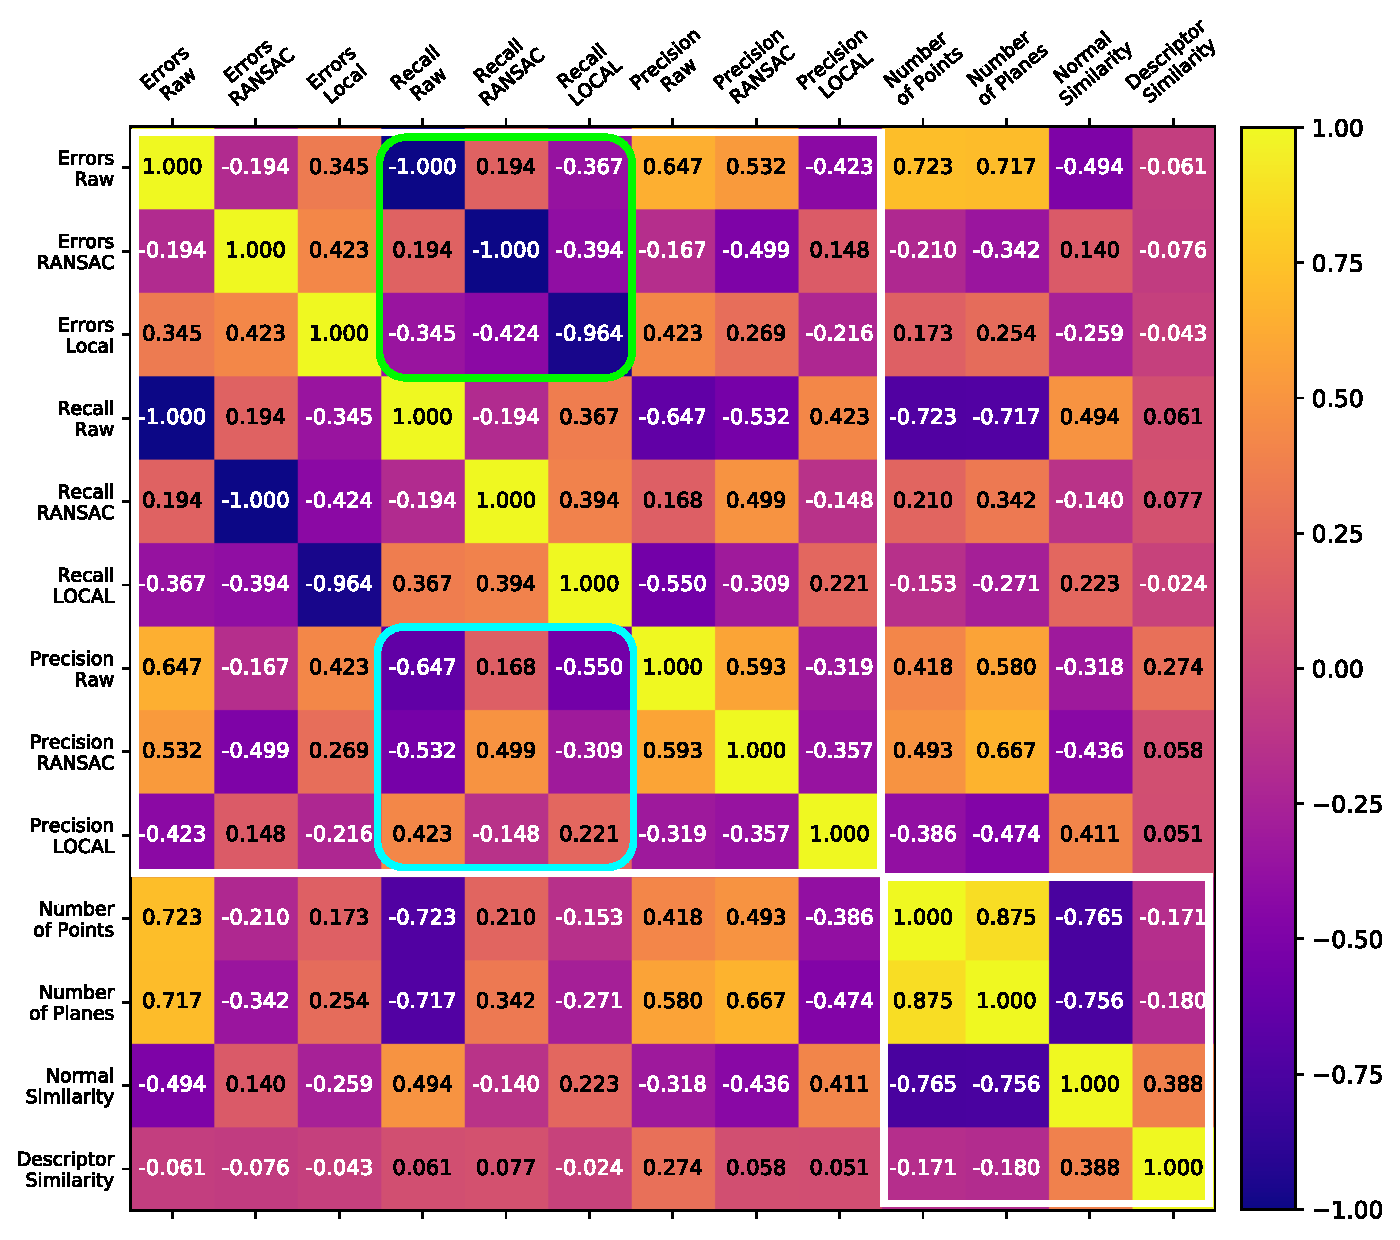
\includegraphics[width=0.99\columnwidth]{figures/plots/space-analysis-corrcoef-more-rotations-all-edited}
	\vspace{-4mm}
	\caption{Correlation coefficient $\rho$ matrix of inference performance metrics with spatial and descriptor properties}
	\vspace{-2mm}
	\label{fig:space-analysis}
\end{figure}

\paragraph{Correlation of metrics and spatial properties.} Fig. \ref{fig:space-analysis} shows the linear correlation coefficient\footnote{We interpret correlation values $|\rho| > 0.7$ as strong, $0.3 <|\rho| \leq 0.7$ as moderate, and $|\rho| \leq 0.3$ as weak.} ($\rho$) matrix of the performance measures -- error rate, recall, and precision -- and the spatial properties -- number of points, number of planes, normal similarity, and descriptor similarity.
%(big upper left white enclosing box)

As we have previously observed in Table \ref{tab:top-10}, the recall values have strong inverse relationship with the average error rate values, i.e. $\left[-0.964,-1\right]$ (green enclosing box). Likewise, the relationship between precision values and error rate varies from a moderate positive relationship (+0.647) to a weak inverse relationship (-0.216). This variation is also reflected in the correlation of the precision and recall values (blue enclosing box) where we start with a moderate inverse relationship (-0.647) for raw-points spaces but becomes weak (+0.221) for locally-generalized spaces. Again, the moderate inverse relationship between precision and recall/error rate for complete spaces is contributed primarily by the errors from partial spaces with smaller radii.

Similarly, linear correlation values between the inference performance and spatial properties provide varying, and inconsistent correlation. If we are only to focus relationships of spatial properties with inference over Raw and RANSAC spaces, there are a few with moderate, direct relationships, i.e. 0.418 (RAW) \& 0.493 (RANSAC) for number of points, and 0.580 (Raw) \& 0.667 (RANSAC) for number of planes). However, for the other spatial properties,  it is not conclusive whether ther affect inference especially over LOCAL spaces. %Thus, with our current 3D spatial dataset, it is not conclusive whether spatial properties -- i.e. number of planes, normal similarity, descriptor similarity -- affect inference. However, i

On the other hand, among the spatial properties themselves, consistent and/or strong relationships can be observed (smaller lower right white enclosing box). Number of points and number of planes obviously have a strong direct relationship, while normal similarity is strongly inversely correlated to both (both have -0.765 correlation). On the other hand, descriptor similarity has a moderate direct correlation to normal similarity (+0.388).%weak inverse correlation to number of points and planes (-0.171 and -0.180, respectively) but has 

\subsection{Computing utility of generalizations}
\label{subsec:utility-results}

% Can we transfer this to an earlier section? In the validation?
% Then just present Privacy vs Utility plots here?

%As we have already emphasized during the discussion on the generalization in \S\ref{subsubsec:generalization} as well as the evaluations in \S\ref{subsec:inference-partials} \& \ref{subsec:inference-successive}, g
Plane-fitting generalizations contribute variations to the released point clouds from true spaces. Fig. \ref{fig:utility} shows the computed average utility based on Eq. \ref{eq:utility-by-sim} for the different generalizations with varying partial radius and acceptability metric $\gamma$. A $\gamma$ value of 1 means that we accept variations for up to 1 unit-combined-difference (see Eq. \ref{eq:utility-by-sim}) of the true point from the released point and the true normal from the released normal. A smaller $\gamma$ value means we do not accept any variations beyond that value; that is, a combined-difference beyond the set $\gamma$ results to a zero utility.

\begin{figure}[t]
	\begin{subfigure}[]{0.595\columnwidth}
		\vspace{-2mm}
    	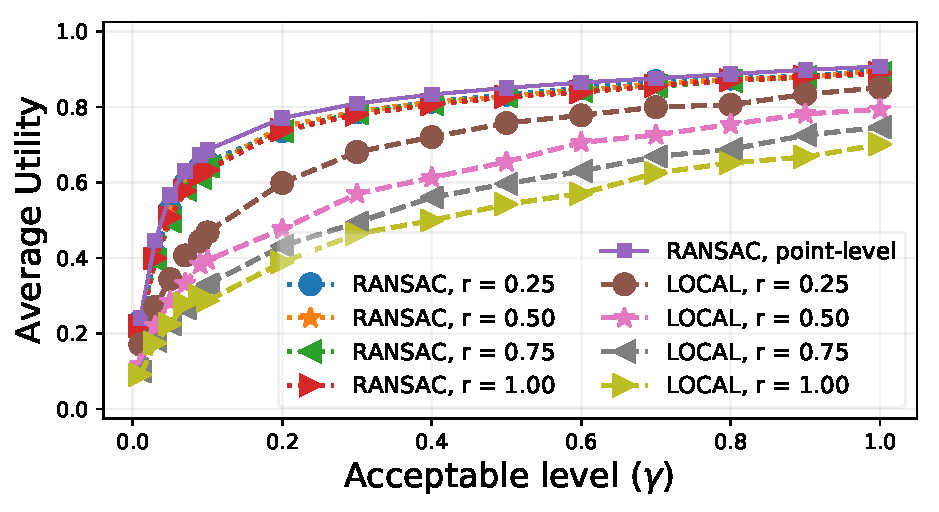
\includegraphics[width=\textwidth]{figures/plots/2-utility}
    	\caption{}
    	\vspace{-2mm}
    	\label{fig:utility}
    \end{subfigure}
    \begin{subfigure}[]{0.395\columnwidth}
    	\vspace{-2mm}
    	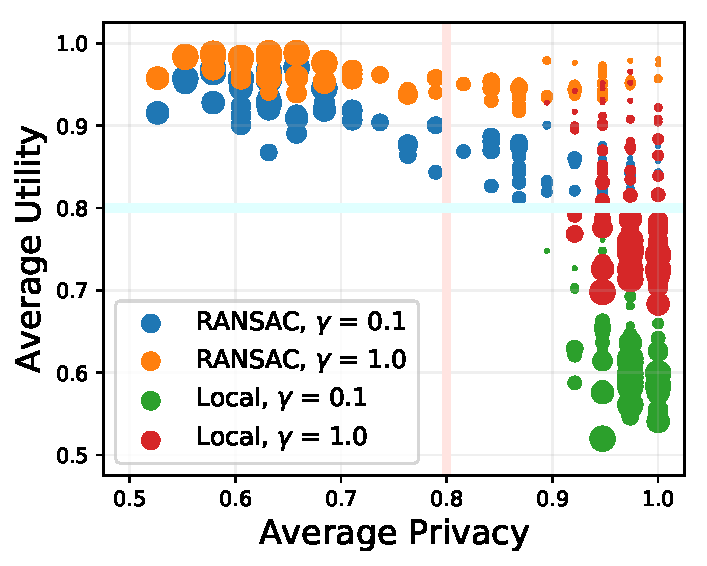
\includegraphics[width=\textwidth]{figures/plots/utility-error-scatter}
    	\caption{}
    	\vspace{-2mm}
	    \label{fig:utility-scatter}
    \end{subfigure}
	\caption{(a) Utility of the generalizations {\small (Note: Utility of true points and planes are always 1.)}; (b) Scatter plot of utility and error rate of different partial spaces (radius is relatively indicated by marker size)}
    \vspace{-3mm}
\end{figure}

For reference, we include the point-level (synonymous to r = 0) utility computation from RANSAC points which produces the highest utility trend, while other RANSAC generalizations of partial spaces with r > 0 comes close second. The average utility provided by RANSAC generalizations are consistent regardless of the size of the released generalized spaces. It does decrease as we decrease the acceptability value $\gamma$, but it does not go too low, i.e $U_{RANSAC} \geq 0.5$ for $\gamma \geq 0.1$, such that the generalizations are rendered unacceptable. This is due to how RANSAC generalizations tries to approach the true spaces.

On the other hand, LOCAL generalizations have lower average utility trends and go much lower as the radius increases. This is due to the increased inaccuracies in the localized generalizations as it disregards point locations and normals other than the randomly chosen origin point for the plane generalization. As a result, the utility trend further decreases as we increase the radius, and this is true for any $\gamma$. In fact, at $\gamma = 0.1$, $U_{LOCAL}\le 0.5$ at r = 0.25. As expected, if we are to set the acceptable utility at $\geq 0.8$, only localized generalizations of radius $r \leq 0.5$ can provide such utility and r = 0.5 barely makes the cutoff at $\gamma = 1.0$. Any $\gamma$ lower than that, only generalizations with $r \leq 0.25$ can provide an average utility $\geq 0.8$.

In reality, these $U_{LOCAL}$ values are unacceptable. If we are to set an acceptability level of $\gamma \leq 0.2$, there is only at most 0.6 chance of getting a locally generalized point that is close to the true point including its orientation. Thus, for the rest of the points from a locally generalized point cloud, augmentations are translated by at most 0.2 meters (in any direction) and/or rotated by at most $cos^{-1}(0.2)$ or $78.5^\circ$.

%The impact of localized generalization is better visualized by its resulting average utility, which decreases as the size of the partial space increases. This is due to the generalization process disregarding point locations and normals other than the randomly chosen origin point for the plane generalization. This decreasing utility trend is true for any $\gamma$. In fact, at $\gamma = 0.1$, the utility is $\le 0.5$ at r = 0.25. In \S\ref{subsec:utility-results}, we further show the impact of generalizations on utility as we change the $\gamma$.

The difference in utility and error rate as we vary the radius of partial spaces is better visualized by the scatter plot in Fig. \ref{fig:utility-scatter}. $U_{RANSAC}$ stays $\geq 0.8$ and privacy drops as we increase the size, while $U_{LOCAL}$ is only $\geq 0.8$ for smaller partial size and the privacy is consistently $\geq 0.8$.

%\begin{figure}[t]
	%\vspace{-2mm}
	%\centering
	%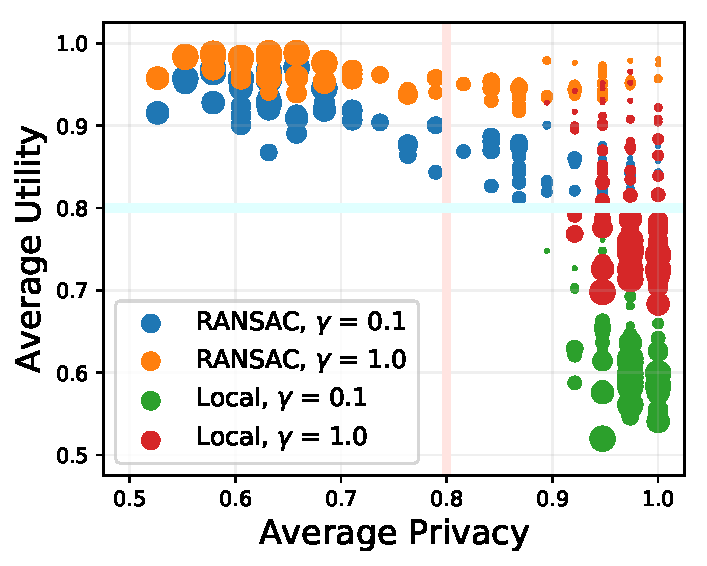
\includegraphics[width=0.65\columnwidth]{figures/plots/utility-error-scatter}
	%\vspace{-2mm}
	%\caption{Scatter plot of utility and error rate of different partial spaces (radius is relatively indicated by marker size)}
	%\label{fig:utility-scatter}
	%\vspace{-3mm}
%\end{figure}

It is also important to note that the utility will be high only for points nearby the reference point of a locally generalized plane as nearby points will most likely have similar normal vector directions. As we go further away from the reference point on the same locally generalized plane, the variation increases and thus the utility drops. In contrast to the RANSAC generalized planes, point location and normal variations are fairly consistent and low regardless of a point's distance from a reference point with which the generalized plane was produced, since it tries to do a good representation of the true space.

\emph{\textbf{Takeaway.}} \textit{Overall, \textbf{LOCAL} generalizations provides high average privacy $(\Pi \geq 0.8)$ but can only provide adequate utility $($i.e. $U$ < 0.5 with $\gamma \leq 0.1)$ with spaces with small radius r $\leq$ 0.25.}

\subsection{Memory compactness of descriptors and inference models}

\begin{figure}[t!]
	\centering
	\vspace{-5mm}
	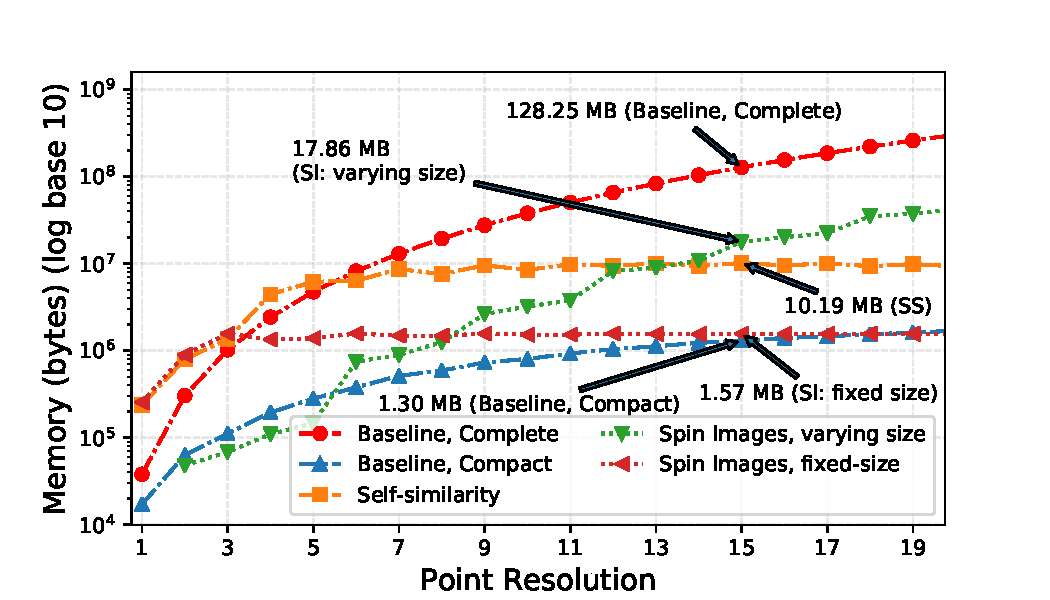
\includegraphics[width=0.75\columnwidth]{figures/plots/2-memory}
	\vspace{-2mm}
	\caption{Used memory by inference models and descriptors extracted from different point cloud resolutions.}
	\label{fig:memory}
	\vspace{-3mm}
\end{figure}

%At $r = 100$, it performs very well with high specificity. Now, we decrease the resolution and compute the error rate. The heatmaps of the reduced resolutions are shown in Fig. \ref{fig:10-90-heatmap}. Starting at resolutions $r \leq 20$, errors start to occur. However, the modelling and processing latencies are about at least two orders of magnitude faster than the inferrer with $r = 100$: $t_{model,r = 100}$  = 103.62 seconds vs $t_{model, r = 20}$  = 0.92 seconds, and $t_{infer, r = 100}$  = 4.24 seconds vs $t_{infer, r = 20}$  = 0.21 seconds.

In the previous sections, we have focused on the inference performance as well as the utility. However, another interesting aspect is how a very good inferrer can still be constructed at a low resolution $res \leq 10$ (Figs. \ref{fig:performance}) with discriminative performance similar to that of higher resolutions. Another remarkable aspect is how the different description and inference model can describe a 3D space dictionary of size 38 which is arguably way more than a usual set of spaces a regular daily user will encounter in a day (assuming we only count the spaces where users spend significant amount of time and where they'd likely to use their MR-capable devices such as their work place, school or class room, bedroom, kitchen, living room, and so on).

Consequently, as shown in Fig. \ref{fig:memory}, the memory size exponentially increases as we increase the resolution. For the rotation-invariant descriptors, if we fix the size of the descriptors, the memory size plateaus.  A baseline Bayesian inference model with a low resolution of 15 requires a memory size of about 128MB. This memory usage is undesirably huge and is due to the almost complete representation of the probabilities in 3D space, which we may represent as a probability cloud. However, we can take advantage of the sparsity of the data points. Empty spaces in the real-world can be represented as zeros in the probability cloud, and, hence, we can just list the non-zero points in the cloud to make it compact.

The memory usage by the compact representation is also shown in Fig. \ref{fig:memory}. A significant reduction in the memory used can be observed. For example, at res = 15, the compact memory usage is now just 1.30 MB from the original 128 MB -- almost 2 orders of magnitude smaller. Thus, an adversarial MR application with access to 3D data produced by the user's MR device can efficiently create a lightweight inference model of the user's space and use it for unintended purposes. (For reference, the original point-cloud data is about 13 MB; thus, our inferrer is a much more compact representation of the point-cloud data at res = 15.)

The same is true for the rotation-invariant descriptors. For the point resolution of res = 15, a corresponding set of self-similarity descriptors takes about 10.19 MB, but a set of corresponding spin image descriptors -- which, anyway, performs better than self-similarity descriptors -- with a fixed descriptor size is as compact as the baseline inference model (that is not rotation-invariant) at only 1.58 MB.

\emph{\textbf{Takeaway.}} \textit{A compact and efficient inferrer of 3D spaces can be created from raw point cloud data released by any MR-capable device (which, now, can be any device with a vision sensor and adequate processing power).}

%\subsection{Analysing the Errors}

% Please add the following required packages to your document preamble:
% \usepackage{booktabs}
%\renewcommand{\arraystretch}{1.4}
%\begin{table}[]
%	\caption{Co relation coefficients of errors with number of points and normal similarity for every space}
%	\label{tab:error_corrcoef}
%	\vspace{-3mm}
%%	\begin{tabular}{@{}ccccc@{}}
%		\cmidrule(l){2-5}
%		\multicolumn{1}{l}{}                                       & \textbf{\begin{tabular}[c]{@{}c@{}}Errors:\\ RANSAC\end{tabular}} & \textbf{\begin{tabular}[c]{@{}c@{}}Errors:\\ Local\end{tabular}} & \textbf{\begin{tabular}[c]{@{}c@{}}Number\\ of Points\end{tabular}} & \textbf{\begin{tabular}[c]{@{}c@{}}Normal\\ Similarity\end{tabular}} \\ 
%		\cmidrule(l){2-5} 
%		\begin{tabular}[c]{@{}c@{}} Errors: Complete\end{tabular} & -0.327                                                                       & 0.484                                                                       & 0.633                                                                          & -0.565                                                                          \\
%		\begin{tabular}[c]{@{}c@{}} Errors: RANSAC\end{tabular}   & -- --                                                                          & 0.088                                                                       & -0.341                                                                         & 0.243                                                                           \\
%		\begin{tabular}[c]{@{}c@{}} Errors: Local\end{tabular}    &                                                                              & -- --                                                                         & 0.219                                                                          & -0.260                                                                          \\
		%\begin{tabular}[c]{@{}c@{}} Number of Points\end{tabular} &                                                                              &                                                                             & -- --                                                                            & -0.765                                                                          \\ 
%		\cmidrule(l){2-5} 
%	\end{tabular}
%\end{table}

\section{Conclusion}\label{sec:conclusion}

%Due to the rise in \textit{mixed reality} (MR) applications and devices in recent years, it is opportune to investigate the privacy and security issues that come with the technology.
In this work, we demonstrated how we can infer and reveal spaces over 3D MR data using existing inference methods, i.e. 3D Bayesian inference and 3D descriptor-based inference. We have utilized 3D point cloud data that have been produced by the Microsoft Hololens. The same point cloud data format is also used by Google's ARCore\footnote{https://developers.google.com/ar/reference/java/arcore/reference/com/\\google/ar/core/PointCloud} and Apple's ARKit\footnote{https://developer.apple.com/documentation/arkit/arpointcloud} which allows us to easily extend this work to these mobile MR platforms. We also demonstrated how leakage can persist even after implementing spatial generalizations. Specifically, RANSAC generalizations can't provide adequate protection especially in the realistic case when successive generalizations are released and exposed to adversaries. On the other hand, LOCAL generalizations provide promise in protecting spatial privacy but utility is currently undesirably low that, if directly applied in actual operation, cause augmentations to be shifted, translated, and/or rotated by a great degree, i.e. maximum average utility of 0.6 for a maximum deviation or error of 0.2 combined-difference\footnote{Combined unit for difference in rotation (cos $\Delta\theta$) and translation ($\Delta x$)}. Improving the LOCAL algorithm's utility while maintaining adequate privacy is a promising endeavor. Moreover, we also present how compact in terms of memory usage these 3D inference models can be which allows adversaries to keep models for every users' set of 3D spaces. Therefore, it is now opportune to start designing and developing privacy-preserving mechanisms for MR that provides quantifiable guarantees and acceptable utility.

%\footnote{https://developers.google.com/ar/reference/java/arcore/reference/com/\\google/ar/core/PointCloud}

%\footnote{https://developer.apple.com/documentation/arkit/arpointcloud}

\section{Related Work}\label{sec:related-work}

In the general privacy and security space, various works have already been done -- from revealing privacy leakage in online social networks \cite{krishnamurthy2010privacy} and mobile devices \cite{ren2016recon}, to developing privacy-preserving mechanisms for conventional user data types \cite{sweeney2002k, mcsherry2007mechanism, dwork2014algorithmic} as well as against deep-learning inference \cite{shokri2015privacy, abadi2016deep}. %Now, we focus on the various privacy-related work in MR.

Most privacy protection techniques for MR were primarily focused on \textit{visual} information or media (i.e. image and video) sanitization \cite{jana2013scanner,raval2014markit, roesner2014world, aditya2016pic, raval2016you, shu2016cardea, li2016privacycamera}. Aside from that are \textit{abstraction} approaches to privacy protection. In the specific 3D use case, significant work have been done on protections involving abstracting physiological information \cite{jana2013scanner, figueiredo2016prepose} using the idea of \textit{least privilege} \cite{vilk2014least}. The same approach has also been used for providing visual privacy when using 3D MR browsers \cite{vilk2015surroundweb};  when actual walls and surfaces are utilized as displays, the 3D browsing applications displayed through them need not know where these surfaces are in the real physical environment; however, it did not specifically protect against spatial inference.

Other recent works have focused on protecting MR outputs specifically in ensuring user safety \cite{lebeck2016safely, lebeck2017securing}. Furthermore, as MR devices allow for new modes of \textit{collaboration}, issues on \textit{power imbalance} brought by the \textit{directionality} of MR interfaces \cite{benford1996shared, benford1998boundaries} are now being studied as well \cite{lebeck2018towards}. A more extensive collection of security and privacy approaches targeting MR are listed and discussed in \cite{deguzman2018security}.

\section{Limitations and Future Work}\label{sec:future_work}
In this work, we have only used \textit{geometric information}, i.e. point location $\{x,y,z\}$ and their normals $\{n_x,n_y,n_z\}$, but point cloud data may also include \textit{photometric information}, such as color, hue, light intensity, and so on. Further extensive analysis and investigation needs to be done over these extensions of the data.

Moreover, we have only employed \textit{classical} inference strategies for this work, i.e. 3D Bayesian inference model, and 3D descriptor matching. There is a great deal of opportunity in improving the inference using other techniques, especially those employed in 3D object detection \cite{xiang2014beyond,yang2018pixor,simon2018complex} and investigate their impact on privacy. In addition, we can also employ a \textit{parrot-matching attack} as used in facial de-identification work \cite{gross2009face}. Also, as future direction, it is imperative to formalize the 3D information measurement so that we can properly and effectively design and develop privacy-preserving mechanisms for 3D and, in general, MR data. Subsequently, we can also formalize a 3D (spatial) privacy metric that informs the design of privacy preserving mechanisms for MR  \cite{ Wagner:2018:TPM:3212709.3168389}. Afterwards, we can incorporate a \textit{tunable} privacy-utility mechanism, aside from incorporating \textit{context-awareness} \cite{grubert2017pervasiveAR} and other \textit{user-centric} designs for MR technology.

%Thus, we aim to present a mechanism that enables the denaturization or the transformation of the give 3D data to a privacy-preserving version.
%Future work, context-awareness informs the user as well as the application the possible privacy level or information specificity provided by the users to the apps.
%Future, future work, allows the sharing of 3D information for crowd-sourced 3D services that learns which features of the recorded 3D space are user-sensitive.

 %[...] Specifically, in 3D browsing, actual walls and surfaces are utilised as displays, and the browsing applications displayed through them need not know where these surfaces are in the real physical environment. Another abstraction-based PET focuses on user gesture detection for using gestures as user inputs. ...

%However, it is the \textit{trusted} platform, where the abstractions are usually implemented, that ensures, maintains, and controls utility of the information released to untrusted third party applications and services. If not, then, a necessary reputation-based core has to be in place to ensure reliability of abstractions, whether in the input- or output-side.

\section*{Acknowledgments}  The authors would like to thank *** for providing insights through application activity and network packet analysis of MR applications running in HoloLens, Android's ARCore, and Apple's ARKit.
%  Dr. Yuhua Li for providing the
%  MATLAB code of the \textit{BEPS} method.
%
%  The authors would also like to thank the anonymous referees for
%  their valuable comments and helpful suggestions. The work is
%  supported by the \grantsponsor{GS501100001809}{National Natural
%    Science Foundation of
%    China}{http://dx.doi.org/10.13039/501100001809} under Grant
%  No.:~\grantnum{GS501100001809}{61273304}
%  and~\grantnum[http://www.nnsf.cn/youngscientists]{GS501100001809}{Young
%    Scientists' Support Program}.

\begin{appendix}

\section{3D Description Algorithms}\label{apdx:descriptors}

\subsection{Self-similarity-based 3D descriptors}\label{apdx:self-similarity}

\begin{figure}[htbp]
	\vspace{-2mm}
	\centering
	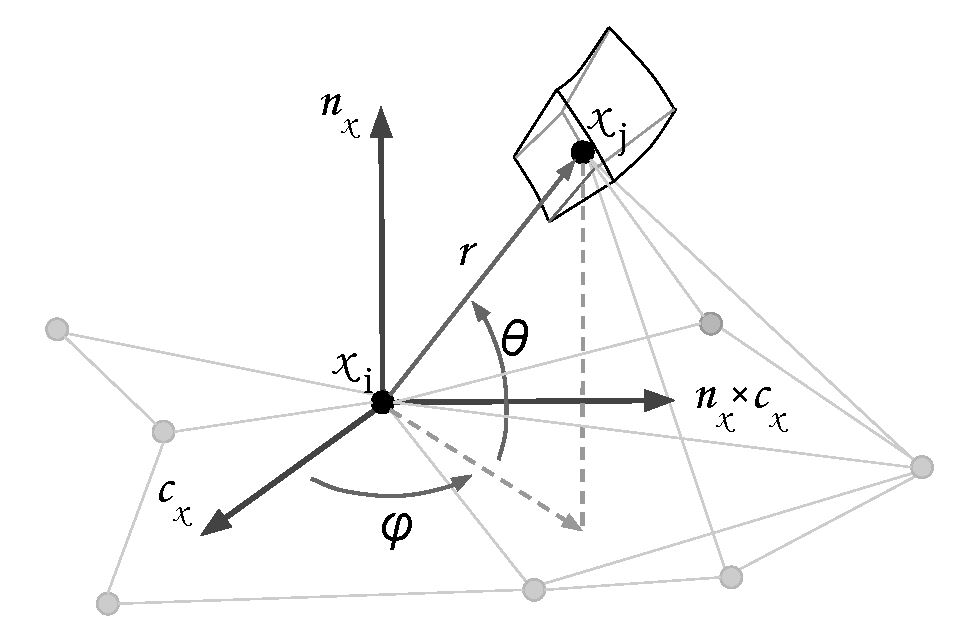
\includegraphics[width=0.65\columnwidth]{figures/spherical-coord}
	\caption{Local spherical coordinate system for self-similarity descriptors}
	\label{fig:spherical-coordinate}
\end{figure}

The description process of the self-similarity-based 3D descriptor \cite{huang2012point} starts with the computation of the local point $x_i$'s self-similarity with its neighbours,
\begin{equation}
N_{x_i} = \{x_j, j \neq i : |x_i - x_j| < r\}
\end{equation}
within a pre-defined neighbourhood radius $r$ (we set $r =$ 1). We compute the local self-similarity of a point as follows:
\begin{equation}
local_{sim} (x_i) = \mean_{\forall x_j \in N_{x_i}}  \left[ \alpha \cdot normal_{sim, x_i} + \beta \cdot curv_{sim, x_i} \right],
\end{equation}
where $\alpha$ and $\beta$ are similarity coefficients (which can be bounded by $\alpha + \beta =1$, be set to $\alpha = \beta = 0.5$), and
\begin{equation}
normal_{sim} = \left[ \pi - cos^{-1}(\vec{n_{x_i}} \cdot \vec{n_{x_j}}) \right] /\pi
\end{equation}
and
\begin{equation}
curv_{sim} = 1 - |\vec{c_{x_i}} -  \vec{c_{x_j}}|.
\end{equation}

Then, a point is chosen as a key point if its curvature is a local maxima. For every chosen key point, a spherical descriptor is computed using the self-similarity. To introduce rotation-invariance, a local coordinate reference as shown in Figure \ref{fig:spherical-coordinate} is computed: the key point $x_i$ is set as the origin, the \textit{z-axis} is the normal vector $\vec{n_{x_i}}$, the \textit{x-axis} is the direction of the principal curvature vector $\vec{c_{x_i}}$, and the \textit{y-axis} is the cross product of $\vec{n_{x_i}} \times \vec{c_{x_i}}$. The local reference system is used to create a binned spherical descriptor {$(r,\phi,\theta)$}. We follow the binning from the reference paper which uses Bin($r$) = 6 radial, Bin($\phi$) = 8 longitudinal, and Bin($\theta$) = 6 latitudinal. Finally, these bins are then filled by the average local self-similarity of the points that fall within the bins and is within a specified spherical local region from the key point. For our implementation, we set the local spherical region to be r = 1 unit. These results to a 3D self-similarity descriptor with dimension 6$\times$8$\times$6. The resulting descriptors are maximum-normalized which makes the highest descriptor value to be 1.

\subsection{Spin Image 3D descriptors}\label{apdx:spin-image}

\begin{figure}[t!]
	\vspace{-2mm}
	\centering
	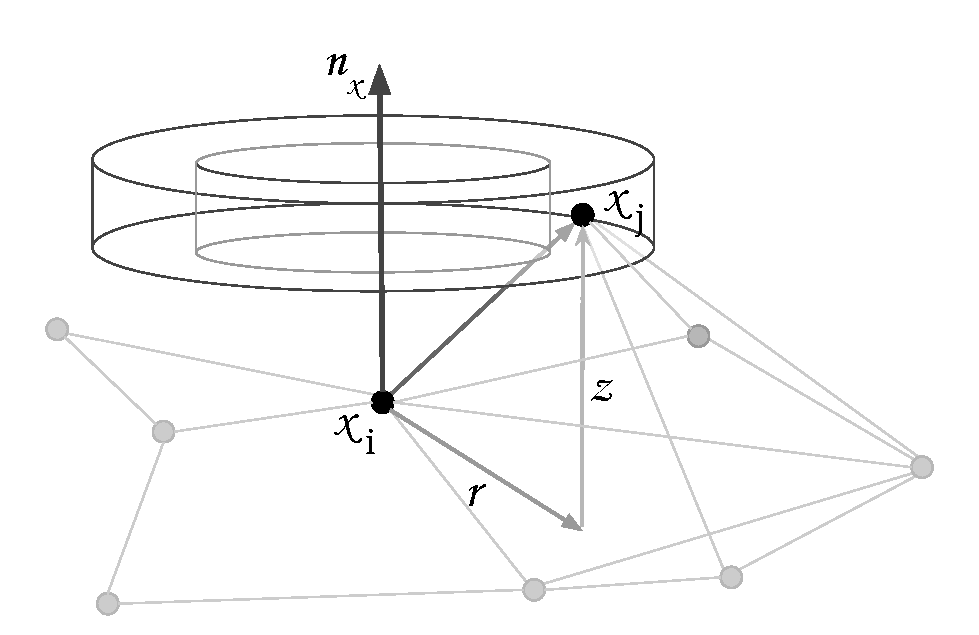
\includegraphics[width=0.65\columnwidth]{figures/cylindrical-coord}
	\caption{Local cylindrical coordinate system for spin image descriptors}
	\label{fig:cylindrical-coordinate}
\end{figure}

The original spin image descriptor algorithm does not have a key point selection process \cite{johnson1998surface,johnson1999using}. For our implementation, we implement a pseudo key point selection process by using a sub-sampled point cloud space (sampling factor of 3) as our chosen key points instead of the complete point cloud. This reduces the likelihood of having neighbouring points having exactly the same descriptors. Then, to compute the descriptor for every key point, we create a local cylindrical $(r,z)$ coordinate system as shown in Figure \ref{fig:cylindrical-coordinate} with the key point $x_i$ as the origin and the normal vector $\vec{n_{x_i}}$ as the \textit{z-axis}. From the local cylindrical coordinate system, a binned descriptor with Bin($r$) = 10 radial bins, and Bin($z$) = 20 (10 for +z direction, and another 10 for -z direction) latitudinal/elevation bins are filled with the number of points that fall within the $(r,z)$ bins. The \textit{spin} comes from the fact that spinning the key point about its normal ($\phi_{cylindrical} 
\in \{0,2\pi\}$) will have no effect on the computed descriptor. Similarly, we also maximum-normalize the spin image descriptors to make the highest value be 1.

\section{Plane Generalization}\label{apdx:generalization}

Our RANSAC plane generalization, shown in Alg. \ref{alg:ransac}, mainly follows the described algorithm in \cite{fischler1981random} except for the normal estimation which we skip and instead use the estimated normal vectors directly provided by the spatial mesh produced by the Hololens.

\begin{algorithm}[htbp]
    \small
	\DontPrintSemicolon
	\textbf{F} the number of planes to find = 30\;
	\textbf{T} the point-plane distance threshold = 0.05\;
	\textbf{R} the number of RANSAC trials = 100\;
	\KwData{$X = \{x_1 , x_2 , ..., x_n\}$, a set of 3D points}
	
	\KwResult{$P = \{p_{x_m} : \{x_{p_1}, x_{p_2}, ...\}\}$, a set of planes (a 3D point, and a normal) and their associated co-planar points}
	\BlankLine
	\For{$f \leftarrow 1$ \KwTo F}{
		bestPlane = $\{0,0\}$\;
		bestPoints = $\{\}$\;
		\For{$r \leftarrow 1$ \KwTo R}{
			$S = {s_1} =$ a point at random from X\;
			$thisPlane = \{s_1 , normal_{s_1}\}$\;
			$thisPoints = \{\}$\;
			\For{$x_i \in X$}{
				\If{(distance($thisPlane , x_i $) $\le$ T)\label{alg:point-test}}
				{$thisPoints \leftarrow thisPoints + x_i$}
			}
			\If{$|thisPoints| > |bestPoints |$\label{alg:plane-test}}{bestPlane $\leftarrow$ thisPlane \; bestPoints $\leftarrow $ thisPoints}
		}
		$P \leftarrow P + \{bestPlane,coPlanarTransformed(bestPoints)\}$\;
		$X \leftarrow X - bestPoints$\;
	}
	\caption{RANSAC algorithm \cite{fischler1981random}}
	\label{alg:ransac}
\end{algorithm}

On the other hand, the algorithm for the locally-originated plane generalization, shown in Alg. \ref{alg:local-plane}, is a crude and simplified generalization which removes the point (Line \ref{alg:point-test}) and plane (Line \ref{alg:plane-test}) discrimination process from RANSAC.

\begin{algorithm}[t]
    \small
	\DontPrintSemicolon
	\textbf{F} the number of planes to find = 30\;
	\textbf{r} the radius of the local region (e.g. 0.5)\;
	\KwData{$X = \{x_1 , x_2 , ..., x_n\}$, a set of 3D points}
	
	\KwResult{$P = \{p_{x_m} : \{x_{p_1}, x_{p_2}, ...\}\}$, a set of planes (a 3D point, and a normal) and their associated co-planar points}
	\BlankLine
	\For{$f \leftarrow 1$ \KwTo F}{
		$S = {s_1} =$ a point at random from X\;
		$thisPlane = \{s_1 , normal_{s_1}\}$\;
		$thisPoints = \{x_i \in X: |x_i - s_1| \leq r\}$\;
		
		$P \leftarrow P + \{thisPlane,coPlanarTransformed(thisPoints)\}$\;
		$X \leftarrow X - thisPoints$\;
	}
	\caption{Locally-originated plane generalization}
	\label{alg:local-plane}
\end{algorithm}

\end{appendix}




%-------------------------------------------------------------------------------
\bibliographystyle{plain}
\bibliography{bib_all.bib}

%%%%%%%%%%%%%%%%%%%%%%%%%%%%%%%%%%%%%%%%%%%%%%%%%%%%%%%%%%%%%%%%%%%%%%%%%%%%%%%%
\end{document}
%%%%%%%%%%%%%%%%%%%%%%%%%%%%%%%%%%%%%%%%%%%%%%%%%%%%%%%%%%%%%%%%%%%%%%%%%%%%%%%%

%%  LocalWords:  endnotes includegraphics fread ptr nobj noindent
%%  LocalWords:  pdflatex acks
